%%
%% Copyright (C) 2010 by Andreas Dräger
%% ... (license header) ...
%%
\documentclass[ % MUST BE THE VERY FIRST COMMAND
  a4paper,                % Paper size
  12pt,                   % Base font size
  headsepline,            % Line under header
  numbers=noenddot,       % Chapter/section numbers without trailing dot
  captions=oneline,       % One-line captions if they fit
  captions=tableheading,  % Table captions above table (KOMA style)
  BCOR=12mm,              % Binding correction
  headinclude,            % Header part of type area calculation
  chapterprefix,          % Use "Chapter X" prefix
  appendixprefix,         % Use "Appendix X" prefix
  index=totoc,            % Add index to table of contents
  bibliography=totoc      % Add bibliography to table of contents
]{scrbook}

% --- Essential Setup ---
\usepackage[utf8]{inputenc} % Input encoding. CRITICAL.
\usepackage[T1]{fontenc}    % Output font encoding. CRITICAL.
\usepackage[ngerman, english]{babel} % Language support. CRITICAL, load ONCE here.


\usepackage{amsmath} % <--- Needed for \textsubscript
\usepackage{booktabs}
\usepackage{multirow}
\usepackage{rotating} % Although not used for these tables, might be needed elsewhere
\usepackage{graphicx}
\usepackage{subcaption}
\usepackage{caption}
\usepackage{geometry} % Optional, for margins
\usepackage{hyperref} % For \href if used elsewhere, though not in table notes now
\usepackage{scrhack}

% --- Custom Dissertation Style ---
% Loads most packages as defined in dissertation.sty
\usepackage{dissertation}

% --- Packages NOT loaded by dissertation.sty ---
\usepackage{siunitx}        % REQUIRED. Load explicitly.
\usepackage{svg}            % REQUIRED. Load explicitly.
\usepackage{ragged2e}       % REQUIRED. Load explicitly.
\usepackage{enumitem}       % REQUIRED. Load explicitly.
\usepackage{threeparttable} % REQUIRED. Load explicitly for tables with notes (\tnote).
\usepackage{makecell}       % REQUIRED. Load explicitly for multi-line cells.

\usepackage{cleveref} % For smarter referencing like \cref{}
\usepackage[version=4]{mhchem}

% --- SIunitx Configuration ---
\DeclareSIUnit{\year}{yr}
\DeclareSIUnit{\hour}{h}
\DeclareSIUnit{\liter}{L}
\sisetup{
  separate-uncertainty = true,
  table-align-uncertainty = true,
  table-align-exponent = false,
}

% --- Robustify Commands ---
% \robustify{\pm} % <<<--- COMMENTED OUT FOR NOW to avoid 'not a macro' error.

% --- Hyperref Setup ---
% Apply detailed settings AFTER hyperref has been loaded by dissertation.sty
\hypersetup{ % <<<--- THIS BLOCK BELONGS HERE
    bookmarksopen={true},
    bookmarksopenlevel={0},
    bookmarksnumbered={true},
    breaklinks={true},
    colorlinks={false},
    pdfborder={0 0 0},
    linkcolor={blue},
    citecolor={blue},
    urlcolor={blue},
    pdfpagemode={UseOutlines},
    pdftitle={\thethesis},
    pdfauthor={\thename},
    pdfsubject={Dissertation},
    pdfkeywords={\thekeywordlist},
    pdfview={FitV},
    pdffitwindow={true},
    pdfstartview={FitV},
    pdfnewwindow={false},
    pdfdisplaydoctitle={true},
    plainpages={false},
    unicode={true}
}

% --- KOMA-Script Compatibility ---
% Load scrhack late. MUST be loaded explicitly.
\usepackage{scrhack}

% --- Metadata Setup ---
% CALL the commands defined in dissertation.sty to set document specifics.
% <<<--- THIS BLOCK BELONGS HERE
\degree{M.Sc.}
\name{Nicolás Riveras Muñoz}
\thesis{Biological soil crust and climate effects on soil stabilization, erosion, and nutrient dynamics across the Chilean Coastal Range}
\keywordlist{list, of, comma, separated, keywords}
\hometown{Puente Alto}
\dean{Prof.~Dr.~Thilo Stehle}
\reviewerone{Prof.~Dr.~Thomas Scholten}
\reviewertwo{Dr.~Peter Kühn}

% \doublespacing

% --- Hyphenation ---
\selectlanguage{english}
\hyphenation{
con-cen-tra-ti-ons
Bio-crusts
bio-crusts
}

% --- Title Page Setup ---
\title{\thethesis}
\author{\Large Dissertation\\ % Content for the author field
\normalsize der Mathematisch-Naturwissenschaftlichen Fakult\"at\\
\normalsize der Eberhard Karls Universit\"at T\"ubingen\\
\normalsize zur Erlangung des Grades eines\\
\normalsize Doktors der Naturwissenschaften\\
\normalsize (Dr.~rer.~nat.)}
\date{\ \\[2ex]\normalsize vorgelegt von\\ % Content for the date field
\thedegree~\thename\\
\normalsize aus \thehometown}
\publishers{\normalsize T\"ubingen\\\normalsize 2025} % Content for the publishers field
\lowertitleback{ % Content for the back of the title page
    Gedruckt mit Genehmigung der Mathematisch-Naturwissenschaftlichen Fakult\"at der
    Eberhard Karls Universit\"at T\"ubingen. \\ \\ \\
    \begin{tabular}{@{}lp{.8\textwidth}@{}}
    Tag der m\"undlichen Qualifikation:& XX.XX.2025\\
    Dekan:                             & \thedean\\
    1.~Berichterstatter:               & \thereviewerone\\
    2.~Berichterstatter:               & \thereviewertwo\\
\end{tabular}}

% --- Selective Compilation ---
% \includeonly{tex/Introduction, tex/Methodology}

% ==============================================================================
\begin{document} % <<<--- MARKS THE START OF THE ACTUAL DOCUMENT CONTENT
% ==============================================================================

\frontmatter
% \selectlanguage{ngerman} % Usually not needed here unless \maketitle uses language-specific terms
\maketitle
\selectlanguage{english} % Ensure English is active for main content

% --- Front Matter Sections ---
% \chapter*{Abstract}
\markboth{Abstract}{Abstract}

Biological soil crusts (biocrusts) and climate effects profoundly shape soil stabilization, erosion, and nutrient dynamics, especially across diverse environmental gradients like the Chilean Coastal Range (arid to humid). This research explored these intricate interactions by integrating field observations, rainfall simulations, laboratory experiments, and advanced analytical techniques. The focus was on the interplay between biocrusts, microbial communities, plant roots, and fundamental soil properties.

Key findings reveal that biocrusts significantly enhance soil aggregate stability, particularly in drier regions, thereby reducing surface runoff and erosion. Their stabilizing influence, however, lessens in humid climates where dense vegetation becomes the dominant factor. Biocrusts modify hydrological pathways, typically decreasing surface flow while sometimes increasing percolation. They also modulate carbon (C) and nitrogen (N) fluxes in climate-dependent ways, influencing both sediment-bound and dissolved nutrient transport.

The critical role of microbial communities in soil aggregation and development was confirmed, with their activity and resilience strongly linked to climate legacy and moisture patterns (e.g., wetting-drying cycles). Plant roots emerged as powerful drivers of macroaggregation, exerting distinct influences during their living (rhizosphere) and decaying (detritusphere) phases, which in turn affects microbial succession and organic matter protection. Overall, this work highlights the interconnected, context-dependent nature of these biotic and abiotic factors in governing soil structure and function.


% \selectlanguage{ngerman}
% \chapter*{Kurzfassung}
\markboth{Kurzfassung}{Kurzfassung}

\begin{justify}
Biologische Bodenkrusten (Biokrusten) und Klimaeffekte prägen maßgeblich die Bodenstabilisierung, Erosion und Nährstoffdynamik, insbesondere entlang diverser Umweltgradienten wie der chilenischen Küstenkordillere (arid bis humid). Diese Forschung untersuchte diese komplexen Wechselwirkungen durch die Integration von Feldbeobachtungen, Regensimulationen, Laborexperimenten und fortschrittlichen Analysetechniken. Der Fokus lag auf dem Zusammenspiel zwischen Biokrusten, mikrobiellen Gemeinschaften, Pflanzenwurzeln und grundlegenden Bodeneigenschaften.

Wichtige Ergebnisse zeigen, dass Biokrusten die Aggregatstabilität des Bodens signifikant erhöhen, besonders in trockeneren Regionen, wodurch Oberflächenabfluss und Erosion reduziert werden. Ihr stabilisierender Einfluss nimmt jedoch in humiden Klimazonen ab, wo dichte Vegetation zum dominierenden Faktor wird. Biokrusten modifizieren hydrologische Pfade, indem sie typischerweise den Oberflächenabfluss verringern, während sie manchmal die Perkolation erhöhen. Sie modulieren auch Kohlenstoff- (C) und Stickstoff- (N) Flüsse auf klimaabhängige Weise und beeinflussen sowohl den sedimentgebundenen als auch den gelösten Nährstofftransport.

Die entscheidende Rolle mikrobieller Gemeinschaften bei der Bodenaggregation und -entwicklung wurde bestätigt, wobei ihre Aktivität und Resilienz stark mit Klima-Legacy-Effekten und Feuchtemustern (z.B. Benetzungs-Trocknungs-Zyklen) verknüpft sind. Pflanzenwurzeln erwiesen sich als starke Treiber der Makroaggregation, die während ihrer lebenden (Rhizosphäre) und zerfallenden (Detritussphäre) Phasen unterschiedliche Einflüsse ausüben, was wiederum die mikrobielle Sukzession und den Schutz organischer Substanz beeinflusst. Insgesamt hebt diese Arbeit die vernetzte, kontextabhängige Natur dieser biotischen und abiotischen Faktoren bei der Steuerung von Bodenstruktur und -funktion hervor.
\end{justify}
% \selectlanguage{english}
% \include{tex/Acknowledgments}

% --- Tables of Contents, Figures, Tables ---
\tableofcontents
% \listoftables
% \listoffigures

% --- List of Publications ---
\chapter*{List of publications}
\markboth{List of publications}{List of publications}

\begin{enumerate}

\item \textbf{Riveras-Muñoz, N.}; Seitz, S.; Witzgall, K.; Rodríguez, V.; Kühn, P.; Mueller, C. W.; Oses, R.; Seguel, O.; Wagner, D.; and Scholten, T. (2022): Biocrust-linked changes in soil aggregate stability along a climatic gradient in the Chilean Coastal Range. \textit{SOIL}, 8, 717--731. DOI: \href{https://doi.org/10.5194/soil-8-717-2022}{10.5194/soil-8-717-2022}.

\item \textbf{Riveras-Muñoz, N.}; Seitz, S.; Gall, C.; Rodríguez, V.; Witzgall, K.; Kühn, P.; Mueller, C.W.; Oses, R.; Seguel, O.; Wagner, D.; Scholten, T. (submitted): Biocrusts as climate-dependent regulators of erosion, water and nutrient cycling. \textit{Geoderma}.

\item Rodríguez, V.; Bartholomäus, A.; Witzgall, K.; \textbf{Riveras-Muñoz, N.}; Oses, R.; Liebner, S.; Kallmeyer, J.; Rach, O.; Mueller, C.W.; Seguel, O.; Scholten, T. and Wagner. D. (2024): Microbial impact on initial soil formation in arid and semiarid environments under simulated climate change. \textit{Frontiers in Microbiology}, 15:1319997. DOI: \href{https://doi.org/10.3389/fmicb.2024.1319997}{10.3389/fmicb.2024.1319997}.

\item Mitzscherling, J.; Oses, R.; \textbf{Riveras-Muñoz, N.}; Mueller, C. W.; Seguel, O. and Kühn, P.; Scholten, T. and Wagner, D. (2024): Microbially Induced Soil Aggregate Turnover Across Different Climates and Moisture Regimes. SSRN: DOI: \href{https://doi.org/10.2139/ssrn.4740477}{10.2139/ssrn.4740477}.

\item Witzgall, K.; Steiner, F.A.; Hesse, B.D.; \textbf{Riveras-Muñoz, N.}; Rodríguez, V.; Teixeira, P.P.C.; Li, M.; Oses, R.; Seguel, O.; Seitz, S.; Wagner, D.; Scholten, T.; Buegger, F.; Angst, G.; Mueller, C.W. (2024): Living and decaying roots as regulators of soil aggregation and organic matter formation---from the rhizosphere to the detritusphere. \textit{Soil Biology and Biochemistry}, 197, 109503. ISSN 0038-0717. DOI: \href{https://doi.org/10.1016/j.soilbio.2024.109503}{10.1016/j.soilbio.2024.109503}.

\end{enumerate}


\mainmatter

% --- Main Content Chapters ---
\chapter{Introduction}
\section{Biological soil crusts and soil aggregate stability along a climatic gradient}
\label{sec:BiocrustAndStabilityInCLimate}

Life has deeply shaped the surface of Earth over billions of years, actively modifying its environment within the Critical Zone--Earth's living skin--which forms the dynamic interface between the lithosphere, atmosphere, hydrosphere, and biosphere \citep{Amundson2007,Brantley2017,Dietrich2006}. The soil, a central component of this zone, mediates essential biogeochemical processes and supports terrestrial ecosystems. Although soil is subject to constant reshaping by erosion, weathering, and tectonic activity \citep{Scholten2017}, organisms, particularly biological soil crusts (biocrusts), significantly influence its structural integrity and stabilization.

Biocrusts are formed from complex interactions among diverse organisms, including photoautotrophs such as cyanobacteria, algae, lichens, and bryophytes, and heterotrophs such as bacteria, fungi, and archaea, which intertwine with soil particles through their own filamentous structures and polysaccharide-based adhesives \citep{Belnap2016,Gao2017,Weber2022,Xiao2022}. This intricate biological network establishes a cohesive, mesh-like layer that firmly binds the uppermost soil surface, functioning as a protective, living skin on Earth's surface. Biocrust enhance soil aggregate stability by physically protecting soil aggregates, sheltering organic matter, and facilitating microbial colonization.

The stabilizing role of biocrusts is especially crucial in arid environments, where their drought tolerance and low water requirements make them the predominant biological cover \citep{Chen2020,Oliver2005}. This resilience comes from their ability to remain dormant during extended dry periods, reviving rapidly upon rewetting, even after complete desiccation, a capability attributed to the lack of specialized desiccation control structures like stomata or impermeable cuticles \citep{Maegdefrau1951,Proctor2007,Thielen2021}. Consequently, biocrust water content directly reflects the humidity of the surrounding environment, making them uniquely adapted to arid and semi-arid regions \citep{Colesie2016, Grote2010}. Under these conditions, biocrust-induced soil stability achieves its maximum impact, significantly reducing erosion susceptibility and facilitating soil formation processes.

However, as climate humidity increases along a gradient towards more temperate conditions, vegetation competes more effectively and biocrusts are often relegated to resource-limited niches \citep{Budel2016}. In temperate regions, biocrusts stablishes on bare soils or soils with minimal plant development, where conditions such as high salinity, low nutrient availability, and limited water availability mirror the limiting conditions of arid landscapes \citep{Corbin2020}. Thus, the interplay between biocrusts, microbial communities, and plant roots shifts along this climatic gradient, diminishing, but not eliminating, the protagonism of biocrusts on soil stability, structure and size distribution of soil aggregates.

\section{Microbial communities as drivers of aggregate structure}
\label{sec:MicrobialCommunitiesAggregateStructure}

Soil, far from being an inert substrate, is a dynamic and living entity teeming with a vast, often underappreciated, majority: microbial communities. These microscopic organisms, including bacteria, archaea, fungi, and protists, are the main drivers of soil development and functioning, influencing almost every aspect of terrestrial ecosystems \citep{Bardgett2014}. Their ubiquity and sheer abundance, with cell counts often reaching billions per gram of soil, underscore their significance in biogeochemical processes \citep{Nunan2001}. Microorganisms mediate complex nutrient cycles that involve carbon, nitrogen, and phosphorus, transforming organic matter and making essential elements accessible for plant uptake \citep{Schimel2012}. Furthermore, they actively participate in the weathering of minerals, contributing to soil development and releasing nutrients into the environment \citep{Barkay2001,Burford2003}. Their metabolic activities influence soil pH, redox conditions, and the overall chemical environment, thus creating diverse microhabitats that sustain a wide variety of life forms \citep{Brehm2005}.

The resilience and adaptability of microbial communities is perhaps most strikingly demonstrated in extreme environments. Arid climates, characterized by drastic temperature fluctuations, minimal precipitation, and limited nutrient availability, provide compelling examples of how microbial life thrives under harsh conditions. Research in these arid ecosystems has revealed unexpectedly high abundances of diverse microorganisms, even in extremely dry desert environments \citep{Bernhard2018,Newsham2016}. This ability to withstand environmental stress makes desert soils particularly valuable for understanding the potential effects of climate change on microbial communities \citep{Pearce2012}. Studying these environments offers valuable insights into the limits of life and the adaptive strategies microorganisms employ when confronted with adversity. Such knowledge is invaluable for understanding the potential responses of microbial communities to ongoing and future environmental changes.

The connection between microbes and the development of soil structure is profound. Microorganisms colonize raw mineral substrates such as saprolite or newly formed desert soils, initiating a complex successional process that transforms bare rock into fertile soil \citep{Lazaro2008,Stradling2002}. They contribute to mineral weathering through the production of organic acids and other metabolites that dissolve rock surfaces \citep{Bajerski2013,Mavris2010,Styriakova2012}. Along the Chilean Coastal Range, climate distinctly shapes microbial community composition, driving shifts in microbial functions, including their capability to stabilize soil aggregates \citep{Bernhard2018}. Microbes decompose organic matter derived from plant and animal residues, releasing nutrients and contributing to the formation of soil organic matter, a critical component of soil structure and fertility \citep{Oades1993}. Furthermore, microbial communities actively participate in the formation of soil aggregates by exuding substances like polysaccharides, which act as a glue, binding soil particles together and creating a stable soil structure \citep{Martens1992,SchlechtPietsch1994}. Consequently, climatic-driven microbial succession directly influences soil aggregation, which is essential for maintaining soil stability, enhancing water infiltration, reducing soil erodibility, and ultimately fostering ecosystem development.

\section{Climate as a driver of soil and microbial dynamics}
\label{sec:ClimateMicrobialDynamics}

Climate stands as a primary architect of soil, profoundly influencing its formation, structure, and function \citep{Jenny1941}. Temperature and precipitation regimes, along with evapotranspiration rates, dictate the weathering of parent material, the accumulation and decomposition of organic matter, and the development of distinct soil horizons \citep{Scholten2017}. These climatic factors also exert a strong influence on the soil water balance, which in turn affects nutrient availability and the overall biogeochemical cycling within the soil ecosystem \citep{Eldridge2020,Thielen2021}.

The influence of climate extends beyond the purely abiotic realm, shaping the composition and activity of microbial communities that inhabit the soil \citep{Nemergut2005}. Different climatic conditions select for distinct microbial populations, influencing their functional capabilities and the biogeochemical processes they mediate \citep{Newsham2016}. For instance, arid environments, characterized by low precipitation and high temperatures, harbor specialized microbial communities adapted to these extreme conditions \citep{Pearce2012}. These microbial communities play a vital role in initial soil formation and nutrient cycling, even in the face of resource scarcity \citep{Bernhard2018}. Our own studies in the Chilean Coastal Range revealed distinct patterns in soil properties and microbial communities along a climate gradient \citep{Bernhard2018}. Interestingly, these trends often followed specific, rather than homogeneous, patterns, indicating the presence of threshold processes and buffering mechanisms in soil ecosystems \citep{Bernhard2018}.

The development and distribution of biological soil crusts (BSCs) are also intricately linked to climate. Water availability, driven by precipitation and evapotranspiration, is a major determinant of biocrust cover and composition \citep{Bowker2016}. Arid regions tend to favor biocrust dominance due to the scarcity of vascular plant cover \citep{Colesie2016,Grote2010}, while more humid climates support greater plant diversity, leading to a mosaic of biocrusts interspersed with plants \citep{Issa1999}. The protective effects of BSCs against erosion and their influence on soil hydrology also vary depending on climate, with potential trade-offs between runoff reduction and water infiltration \citep{Thielen2021}. These findings demonstrate the importance of considering climate not only as a driver of soil properties but also as a key factor shaping microbial communities and the distribution and functionality of biocrusts. The Chilean Coastal Range, with its dramatic gradient from arid to humid conditions, provides a natural laboratory for investigating these complex interactions. This gradient allows us to explore how the interplay of climate, soil, microbes, and biocrusts shapes the Earth’s surface across varying environmental conditions. Furthermore, understanding how climate influences these components individually and in combination is crucial for predicting how soil ecosystems will respond to future environmental changes. The non-linear nature of some of these climate-driven changes, coupled with the potential existence of thresholds in soil processes across environmental gradients, highlights the need for comprehensive research in diverse climatic settings \citep{Bernhard2018}.

\section{Influence of plant roots and interactions with biocrusts along the climate gradient}
\label{sec:PlantRootsBiocrust}

Soil, far from being a simple mixture of minerals and organic matter, is a dynamic and intricate web of interactions between diverse biotic and abiotic components. Central to this web are plant roots, which exert a profound influence on the surrounding soil environment, driving structural changes, altering nutrient availability, and shaping microbial communities \citep{Hinsinger2009}. These complex interactions among roots, microbes, and soil particles constitute a fundamental axis supporting soil development and ecosystem functioning.

Roots physically restructure the soil matrix through growth and penetration, creating channels and pores, thereby enhancing aeration and water infiltration \citep{Bruand1996}. This process of bioturbation is particularly relevant in developed soils, where root systems establish intricate networks of interactions with the surrounding environment. Moreover, roots release a variety of compounds, known as rhizodeposits, including sugars, amino acids, and organic acids, which serve as primary substrates for soil microorganisms \citep{Hinsinger2009,Rasse2005}. This concentrated release of labile carbon in the rhizosphere fuels microbial activity, creating a "hotspot" of biological processes \citep{Hinsinger2009}.

The impact of roots, however, extends beyond the immediate vicinity of the living root. As roots senesce and decompose, they enter the detritusphere, a zone characterized by the breakdown of plant-derived organic matter \citep{Vidal2018}. In this zone, the legacy of roots persists as decomposed root material contributes to soil organic matter formation and influences the structure and stability of soil aggregates \citep{Six2004}. The transition from rhizosphere to detritusphere marks a shift in the microbial community, as the readily available carbon from rhizodeposits is replaced by more complex organic compounds derived from decaying root tissues \citep{Vidal2018}. This shift in resource availability triggers microbial succession, favoring microorganisms capable of degrading these more recalcitrant substances.

Importantly, the interactions between biocrusts and vascular plants form a dynamic feedback loop in soil ecosystems. Biocrusts, as early colonizers of bare ground, contribute to the initial stabilization of the soil surface, creating microhabitats that facilitate subsequent plant establishment \citep{BelnapBudel2016,Bowker2006}. As plants colonize and their root systems develop, they further enhance soil structure formation, promoting the accumulation of organic matter, and creating conditions for diverse microbial communities to thrive \citep{Schweizer2018,Six2004}. This positive feedback loop between biocrusts and plants drives the development from initial, unstable soil environments towards more mature and resilient soil ecosystems. Thus, along environmental gradients, plant roots progressively become primary agents of aggregate stability, influenced indirectly but significantly by earlier biocrust colonization and microbial activity.

\section{Biocrusts, hydrological processes, and nutrient fluxes influencing soil erosion}
\label{sec:BiocrustFluxes}

Climatic conditions strongly shape biocrust composition, morphological characteristics, and ecological functions, thus influencing hydrological processes, nutrient cycling, and susceptibility to soil erosion \citep{Belnap2003,ConcostrinaZubiri2014}. In arid environments, biocrusts dominated by cyanobacteria and lichens typically form smooth, compact surfaces enriched with microbial biomass and extracellular polysaccharides (EPS), profoundly affecting surface hydrology \citep{RodriguezCaballero2018,Weber2022}. Such biocrust structures frequently lead to surface pore clogging, potentially increasing runoff initiation but simultaneously reducing sediment loss by enhancing aggregate stability and protecting soil organic matter \citep{Kidron2021}. Conversely, in humid climates, biocrusts with higher proportions of bryophytes and fungi possess rougher surfaces that promote water retention, facilitate infiltration, and reduce runoff, thereby strongly influencing sediment transport and nutrient dynamics \citep{RiverasMunoz2022,Seitz2017}.

These functional differences across climate conditions emphasize the critical role biocrusts play in regulating carbon (C) and nitrogen (N) fluxes, erosion dynamics, and soil fertility. Biocrusts act as initial stabilizers of soil organic matter, even preceding plant colonization, thus shaping early nutrient cycling pathways \citep{Belnap2007,Young2022}. Furthermore, by physically absorbing raindrop energy, trapping sediment, and promoting microbial-driven aggregate formation, biocrusts provide a protective barrier against erosion, influencing water and sediment fluxes \citep{Costa2018,Xiao2022}.

However, the way in which biocrust-mediated hydrological processes, nutrient cycling, and erosion control shift across gradients of temperature and humidity remains uncertain. These functional patterns are complex and nonlinear, reflecting intricate interactions between biocrust structure, microbial activity, vegetation competition, and climatic variability rather than a simple linear climatic transition \citep{Bernhard2018,RiverasMunoz2025}.

\section{Understanding biocrusts across a climatic gradient}
\label{sec:BiocrustClimate}

Soil represents an intricate web of interactions among diverse organisms, where biocrusts play a pivotal climate-dependent role in stabilizing aggregates, regulating erosion, and controlling water and nutrient fluxes. This biocrust-mediated stabilization effect is most pronounced in arid regions due to minimal vegetation, decreasing in relative importance but persisting as climates become more humid. Along the Chilean Coastal Range, this dynamic illustrates how biocrusts, microbial communities, and plant roots co-evolve, shaping soil structure, erosion resistance, and nutrient cycling.

Addressing these complex interactions and feedbacks is crucial for predicting how soils and associated ecosystems will respond to ongoing climate changes, especially considering the non-linear and threshold-driven nature of soil processes across environmental gradients \citep{Bernhard2018,Wang2014}. Future research should deepen understanding of these interactions, exploring quantitative relationships to inform conservation strategies and enhance ecosystem resilience in a rapidly changing world.

Understanding how biocrust functions shift across climatic gradients is critical for predicting soil ecosystem responses to environmental changes. The interactions among biocrusts, microbial communities, and plant roots along these gradients exemplify the inherent complexity and nonlinearity of soil processes \citep{Wang2014}. Biocrusts exert differing influences on soil aggregate stability, soil erodibility, water and nutrient flows, reflecting adaptive responses to variations in moisture availability, temperature, and vegetation cover \citep{Belnap2003,Weber2022}. In arid climates, biocrusts typically dominate soil surfaces, forming protective layers that significantly modulate hydrological processes, sediment transport, and microbial activity, thereby strongly influencing soil structure and organic matter dynamics \citep{Kidron2021,RodriguezCaballero2018}. However, as climatic humidity increases, the interplay between biocrusts and plant roots becomes more intricate, with intensified competition from vegetation altering microbial community composition and reshaping nutrient pathways \citep{RiverasMunoz2022,Seitz2017}. Rather than transitioning gradually, these interactions likely exhibit thresholds and complex feedback loops \citep{Wang2014}, implying that even subtle climatic shifts can substantially modify ecosystem functions \citep{Bernhard2018}. Recognizing these nonlinear responses is critical for predicting how soils—and the ecosystems they sustain—will adapt to current and future climatic changes. Addressing these knowledge gaps through quantitative assessments of biocrust-driven processes is therefore essential for developing effective conservation strategies, promoting soil health, and enhancing ecosystem resilience \citep{BelnapBudel2016,Weber2022}.

\section{Objectives and hypothesis}
\label{sec:ObjectivesHypothesis}

This research forms part of the DFG Priority Program: EarthShape: Earth Surface Shaping by Biota (DFG-SPP 1803), specifically within the subproject Microbial Engineers - Drivers of Earth Surface Development and Stabilization. The subproject aims to understand microbial processes that shape Earth's surface, focusing on the roles microorganisms play and providing a quantitative understanding of the mechanisms and microbial taxa involved under various climate conditions. It addresses these questions by: (i) experimentally investigating how microorganisms alone control the formation and transition of initial soils into resilient ecosystems; and (ii) analyzing the combined influence of microorganisms, biocrusts, and plant roots on soil surface stability and erosion under natural and controlled conditions along climatic gradients.

It is hypothesized that biocrusts enhance soil aggregate stability by physically protecting the soil surface, sheltering organic matter, altering microbial community structures, and modifying water infiltration patterns (Manuscripts 1 and 2). This stabilizing effect is expected to be most pronounced in arid climates, where biocrusts represent the primary soil cover due to minimal vegetation and limited organic matter inputs. With increasing humidity, however, the influence of biocrusts on soil stabilization is predicted to diminish, though it will not disappear entirely, due to greater water availability and competition from vegetation (Manuscript 1).

Furthermore, soil microbial communities are hypothesized to accelerate soil formation processes in arid environments when moisture and temperature conditions are favorable. Responses to simulated climate change are expected to be mediated by soil legacy effects, shaping microbial community structure and interactions over time. Bacterial diversity and adaptation processes likely reflect climatic shifts, providing insight into long-term soil developmental dynamics (Manuscript 3). Microbial communities are also expected to be crucial for soil aggregation by influencing soil structure and stability across different climates and stages of soil development. Specific microbial taxa may differentially influence aggregation processes, with their contributions being modulated by biotic and abiotic factors, including wetting-drying cycles and moisture fluctuations (Manuscript 4).

Roots are hypothesized to promote water-stable macroaggregate formation in topsoil and subsoil, with legacy effects persisting after plant death within the detritusphere (Manuscript 5). Microbial abundance near roots is expected to increase due to labile carbon availability, especially in carbon-poor subsoils. The transition from rhizosphere to detritusphere likely triggers microbial succession, favoring gram-positive bacteria as readily available carbon compounds are replaced by more complex materials. Root-derived organic matter, including rhizodeposits and litter, is presumed to significantly influence organic matter dynamics by facilitating the formation of particulate and mineral-associated organic matter, thereby shaping aggregate formation and biogeochemical processes (Manuscript 5).

Lastly, biocrusts are hypothesized to regulate hydrological processes such as runoff, sediment discharge, and percolation flows, along with associated carbon and nitrogen fluxes, thereby reducing soil erosion irrespective of climatic conditions. However, climate-specific feedbacks among these hydrological processes likely mediate carbon and nitrogen transport within biocrust-dominated ecosystems (Manuscript 2).
To test these hypotheses, the objectives of this thesis were to:
\begin{itemize}
  \item Evaluate the role of biocrusts in soil aggregate stabilization and their regulation of erosion, water, and nutrient fluxes across a climatic gradient in the Chilean Coastal Range, examining how variations in biocrust properties correlate with changes in climate and vegetation cover (Manuscripts 1 and 2).
  \item Examine how soil microbial communities influence aggregate formation and stability under different climatic and moisture regimes, as well as their responses to simulated climate-change scenarios (Manuscripts 3 and 4).
  \item Determine the influence of plant roots on soil structure development, microbial succession, and organic matter dynamics during transitions from rhizosphere to detritusphere, emphasizing their role in soil aggregate formation (Manuscript 5).
\end{itemize}
\chapter{Methodology}

\section{Study sites and experimental setting}
\label{sec:StudysitesAndExperimentalSetting}

In order to assess the climatic effect on soil and its interactions with biocrusts, five study sites distributed between latitudes from \ang{26;6}~S to \ang{37;48}~S and over \SI{1315}{\kilo\meter} were established in the Chilean Coastal Range (Figure \ref{fig:location-map}): Pan de Azúcar National Park (PdA), Santa Gracia Natural Reserve (SG), Quebrada de Talca Private Reserve (QdT), La Campana National Park (LC) and Nahuelbuta National Park (NA), corresponding to arid, coastal semi-arid, inland semi-arid, Mediterranean and humid climates, respectively \citep{Bernhard2018}.

\begin{figure}[H]
	\centering
	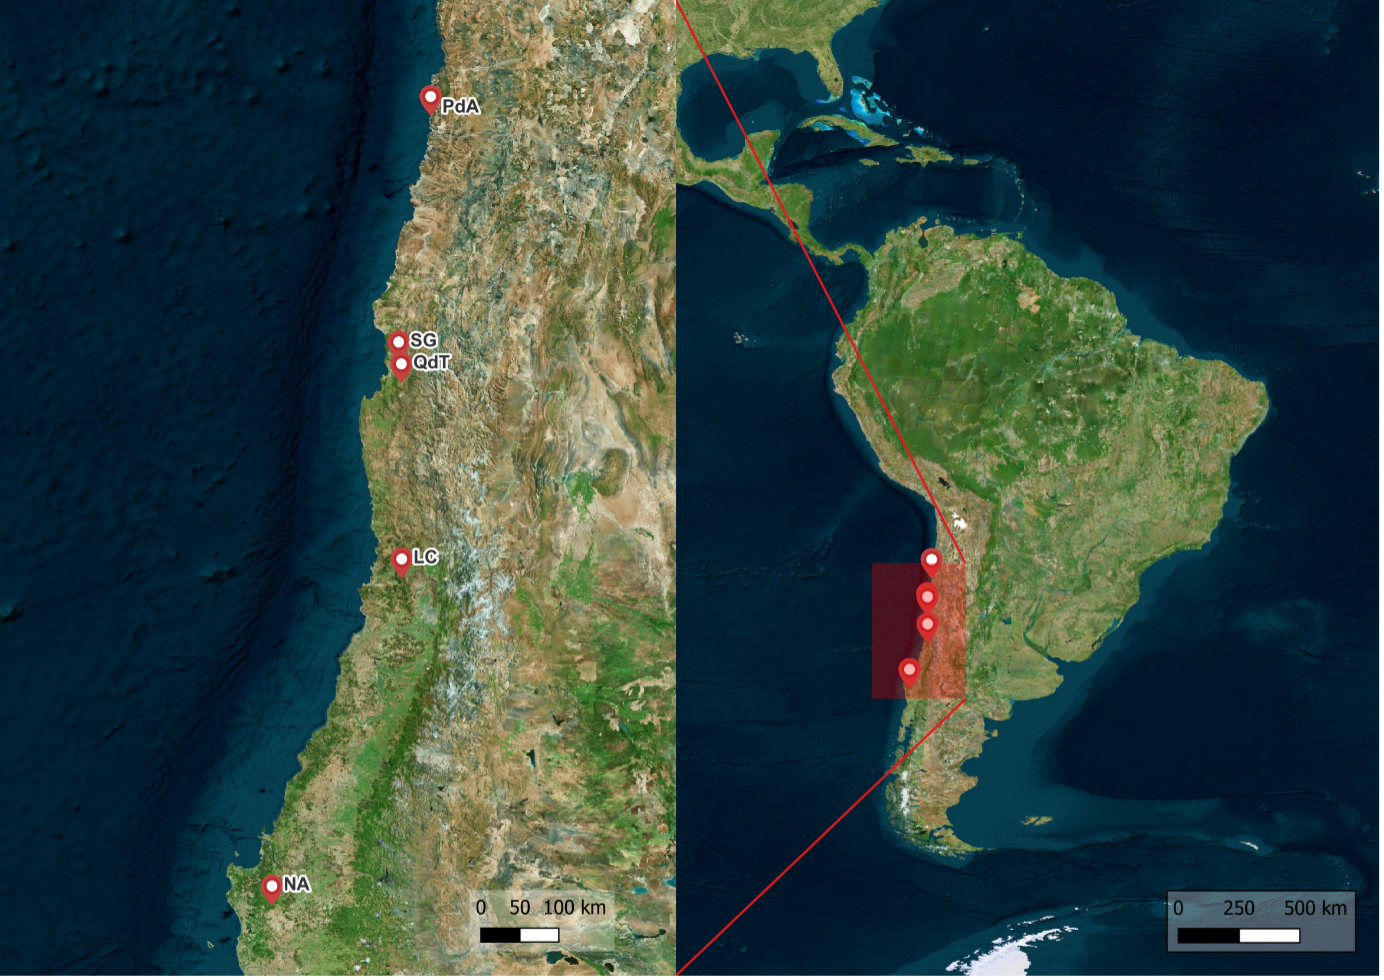
\includegraphics[width=1\textwidth]{img/location-map.png}
	\caption{Location of study sites relative to South America. From north to south: Pan de Azúcar (PdA), Santa Gracia (SG), Quebrada de Talca (QdT), La Campana (LC), and Nahuelbuta (NA).}
	\label{fig:location-map}
\end{figure}

The study sites are comparable in geology, geomorphology, land use, and influence of glaciers and volcanoes \citep{Bernhard2018}. The parent material in all the study sites is granitoid \citep{Bernhard2018}. The dominant topography is generally fluvial valleys, and the sites had no glacial influence during the last glaciation \citep{Hulton2002}. The sites are located within nature protection areas, with limited anthropogenic influence compared to the surrounding areas. Despite this, cattle occasionally enter these locations, and goats, mules, and donkeys have been reported to SG \citep{Armesto2007}.

The mean annual temperature (MAT) decreases from north to south (PdA: \SI{16.8}{\celsius}, SG: \SI{13.7}{\celsius}, QdT: \SI{14.3}{\celsius}, LC: \SI{14.1}{\celsius}, NA: \SI{6.6}{\celsius}). The mean annual precipitation (MAP) in the study sites increases from north to south (PdA: \SI{12}{\milli\metre\,\year^{-1}}, SG: \SI{66}{\milli\metre\,\year^{-1}}, QdT: \SI{109}{\milli\metre\,\year^{-1}}, LC: \SI{367}{\milli\metre\,\year^{-1}}, NA: \SI{1469}{\milli\metre\,\year^{-1}}) with similar rainfall distribution mostly concentrated in winter months (May to August) \citep{Bernhard2018,Santibnez2017}. The elevation of the sites increases from north to south (PdA: \SIrange{329}{351}{\meter}, SG: \SIrange{642}{720}{\meter}, QdT: \SIrange{565}{611}{\meter}, LC: \SIrange{708}{732}{\meter}, NA: \SIrange{1200}{1270}{\meter}). Paleoclimate modeling studies \citep{Mutz2018} indicate that these climate patterns have been persistent since the late Pliocene; thus, the study sites represent the long-term impact of climate on the soil \citep{Ewing2006}. \citet{Bernhard2018} classified soils in the study sites as Regosols in PdA, Cambisols for SG and LC, and Umbrisols in NA. In general, pedogenic properties such as soil depth, clay content, organic matter accumulation, porosity, and activity ratio are positively correlated with site humidity \citep{Bernhard2018}.

For each of the 5 study sites (Figure \ref{fig:location-panel}), 5 plots of \SI{1}{\meter}~$\times$~\SI{1}{\meter} were set up as replicates (P1 to P5). Each plot was assigned in the top-slope position with a south-facing exposition, considering a high presence of site-typical biocrust communities, similar slope and aspect, lack of anthropogenic disturbance, and a maximum distance of \SI{30}{\meter} between each plot. Within each plot, patches with the highest available biocrust cover were included as treatment BSC+, and nearby bare soil without biocrust cover was defined as control (BSC-). \newline

\begin{figure}[h!]
	\centering
	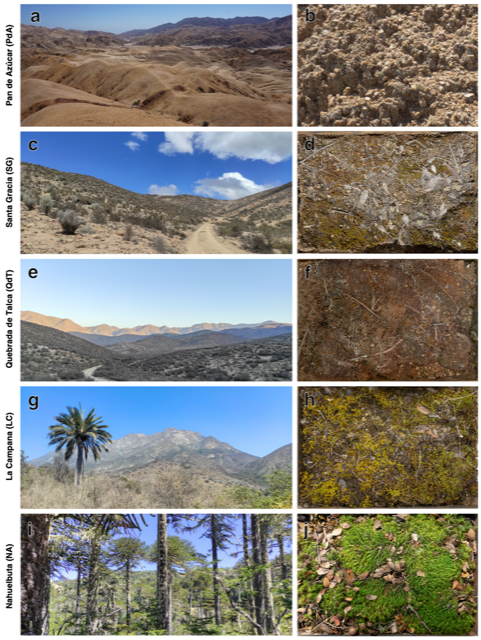
\includegraphics[width=1\textwidth]{img/location-panel.png}
	\caption{General view (a, c, d, g, and i) and sampled biocrust (b, d, f, h, and j) of PdA, SG, QdT, LC, and NA.}
	\label{fig:location-panel}
\end{figure}

\FloatBarrier

\section{Field methods}
\label{sec:FieldMethods}
\subsection{Biocrust sampling and characterization}

In a first field campaign during March 2019, biocrust patches of approximately \SI{100}{\centi\metre^{2}} were collected in PdA, SG, LC and NA and identified according to \citet{Lange2016}. The patches were collected in the field by carefully detaching the biocrust layer, removing the loose soil, and storing it in paper envelopes after air-drying for every research plot. \citet{Samolov2020} describes a biocrusts dominance in PdA with cover of up to 40\%. The other study sites are dominated by higher vegetation that limits the cover of biocrust up to 15\% in SG and 5\% in LC and NA. Sampled communities showed all typical biocrust classes from cyanobacteria, algae, fungi, lichens, liverworts, and mosses. The species composition further showed a graduating change from lichen-dominating biocrusts in the northernmost site to bryophyte-dominating biocrusts in the southernmost site. Biocrusts in NA were specifically found in zones of forest soil disturbance. Bryophyte-dominated biocrusts were sampled with rhizoids down to \SI{5}{\milli\metre} depth; all other communities were down to \SI{2}{\milli\metre}. Dominant macroscopic biocrust species were determined for each of the four sites to the genus level by morphological characteristics using a stereomicroscope (Leitz TS, Wetzlar, Germany), a transmitted-light microscope (Leitz Laborlux S, Wetzlar, Germany), and ultraviolet light. Species groups were separated into bryophytes \citep{Ardiles2014,BednarekOchyra2001,Cuvertino2012,He1998,Lightowlers2013} and lichens \citep{Galloway2007} and assigned to the different regions (Table \ref{tab:taxonomical_composition}). \citet{Bernhard2018}, based on morphological identification of enrichment cultures, reported that the biocrusts of the four studied sites were composed of 18 to 15 species of algae and cyanobacteria; where the richness of green algae increased, while the richness of cyanobacteria decreased with increasing humidity and decreasing mean annual temperature. While \citet{Samolov2020}, based on morphological and molecular traits, reported 18 species in PdA, 26 species in SG, 40 species in LC, and 27 species in NA.

\begin{table}[h!]
\centering
\caption{Taxonomical composition of mosses and lichens in the biological soil crust for the study sites along the climatic gradient.}
\resizebox{\textwidth}{!}{%
\begin{tabular}{lllc}
\hline
\textbf{Site / Division} & \textbf{Family} & \textbf{Genus} & \textbf{No. species} \\
\hline
\textbf{PdA} & & & \\
Lichens & Cladoniaceae & \textit{Cladonia} sp. & 2 \\
        & Verrucariaceae & \textit{Placidium} sp. & 2 \\
        & Lecanoraceae & \textit{Lecidella} sp. & 1 \\
        & Rhizocarpaceae & \textit{Rhizocarpon} sp. & 1 \\
\hline
\textbf{SG} & & & \\
Mosses & Pottiaceae & \textit{Syntrichia} sp. & 2 \\
       & Pottiaceae & \textit{Tortella} sp. & 2 \\
Unidentified lichens & & & 2 \\
\hline
\textbf{LC} & & & \\
Mosses & Bartramiaceae & \textit{Philonotis} sp. & 1 \\
       & Bryaceae & \textit{Bryum} sp. & 1 \\
       & Pottiaceae & \textit{Syntrichia} sp. & 2 \\
       & Pottiaceae & \textit{Tortella} sp. & 2 \\
Unidentified mosses and lichens & & & 2 + 1 \\
\hline
\textbf{NA} & & & \\
Mosses & Amblystegiaceae & \textit{Acrocladium} sp. & 1 \\
       & Amblystegiaceae & \textit{Amblystegium} sp. & 1 \\
       & Bartramiaceae & \textit{Bartramia} sp. & 1 \\
       & Bryaceae & \textit{Bryum} sp. & 1 \\
       & Dicranaceae & \textit{Campylopus} sp. & 2 \\
       & Pterigynandraceae & \textit{Myurella} sp. & 1 \\
Unidentified liverworts, lichens, fungi & & & 2 + 2 + 1 \\
\hline
\end{tabular}}
\label{tab:taxonomical_composition}
\end{table}

\FloatBarrier

\subsection{Soil sampling}

Soil sampling campaigns were primarily conducted during the austral dry season (typically January-April) to capture baseline soil conditions prior to the onset of winter precipitation. Specific sampling approaches were adapted based on the objectives of individual studies. For investigations concerning aggregate stability, moisture regime effects, and general baseline characterization across the full gradient (PdA, SG, LC, NA), bulk topsoil samples (\SIrange{0}{5}{\centi\metre} depth) were collected from each plot on mid-slope, south-facing locations using metal-core augers or by sampling from shallow soil pits (Manuscripts 1 and 4). These samples were processed in the field by sieving ($<$\SI{2}{\milli\metre}), another batch of samples was sieved and sterilized with ethanol, before being homogenized per site or kept discrete per plot depending on the experimental design and subsequently stored at \SI{4}{\celsius} pending laboratory analysis. For studies focusing on initial soil formation and rhizosphere/detritusphere dynamics (PdA, SG), distinct soil horizons (A horizon: \SIrange{0}{2}{\centi\meter}/\SIrange{0}{3}{\centi\meter}; B horizon: \SIrange{2}{3}{\centi\meter}/\SIrange{25}{40}{\centi\meter}) where sampled from excavated soil pits (Manuscripts 3 and 5). Processing involved similar steps: sieving ($<$\SI{2}{\milli\metre}), homogenization per horizon and site, and storage at \SI{4}{\celsius}.

\subsection{Rainfall simulations}

Following observations of limited soil stabilization at PdA, further rainfall simulation experiments were conducted during subsequent expeditions in 2020 and 2022 at SG, Quebrada de Talca (QdT), LC, and NA. Five \SI{1}{\meter}~$\times$~\SI{1}{\meter} plots were established as replicates at each of the four sites, consistently located on south-facing top slopes. Plot selection considered the presence of representative biocrust communities, similar slope and aspect, minimal anthropogenic disturbance, and a maximum inter-plot distance of \SI{30}{\meter}. Within each plot, runoff plots (ROPs) were established in areas with maximum biocrust cover for biocrust-present (BSC+) treatments, and adjacent biocrust-free (BSC-) locations served as controls. The experimental design was a factorial completely randomized design, incorporating four sites (SG, QdT, LC, and NA) (Figure \ref{fig:location-panel}), two biocrust conditions (BSC+ and BSC-), five replicate plots (P1-P5), and three technical replicate ROPs (R1-R3) per plot. This resulted in a total of eight treatments (site × biocrust) with 15 samples per treatment (plot $\times$ technical replicate), yielding a total sample size of n = 60.

Undisturbed soil samples for rainfall simulation were collected (Figures \ref{fig:sampling-panel}b and \ref{fig:sampling-panel}c), using piercing frames (\SI{20}{\meter}~$\times$~\SI{30}{\meter}~$\times$~\SI{7}{\meter}) (Figure \ref{fig:sampling-panel}a) and carefully installed into infiltration boxes to minimize surface and subsurface disturbance (Figure \ref{fig:sampling-panel}d). These steel boxes, designed with a triangular surface runoff gutter and a bottom outlet, captured both runoff and percolated water. Soil water content was measured using a TDR probe (Delta-T Devices Ltd. Cambridge, UK), averaging three measurements adjacent to each ROP. Biocrust cover in BSC+ ROPs was assessed using perpendicular photographs taken with a digital camera (Sony ILCE-6000, SELP1650 lens; Tokyo, Japan). Photographs were analyzed using the grid-quadrat method with a 100-subdivision grid, and biocrusts were identified visually \citep{Belnap2001}.

\begin{figure}[h!]
	\centering
	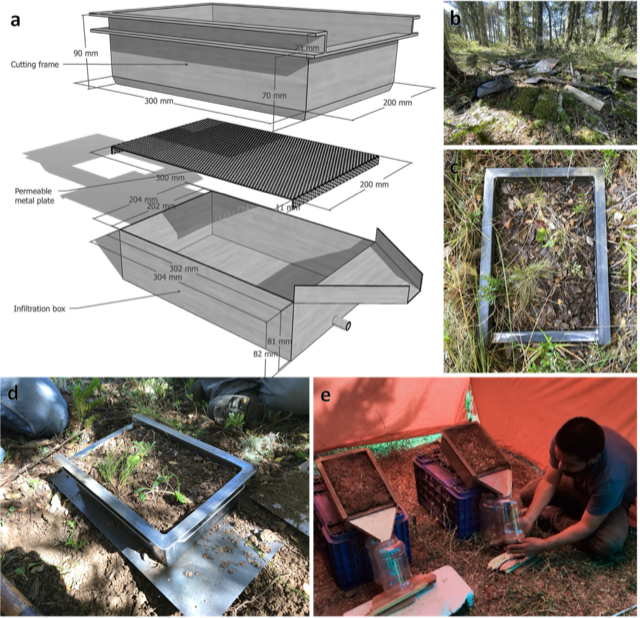
\includegraphics[width=1\textwidth]{img/sampling-panel.png}
	\caption{Construction diagram of the soil erosion flux box used in the experiment (a), general view of a plot with the presence of biocrust prior to sampling (b). (c, d) shows an installed cutting frame and the cleared and prepared soil. (e) demonstrates the setting for rainfall simulations at the Nahuelbuta (NA) study site.}
	\label{fig:sampling-panel}
\end{figure}

\FloatBarrier

Rainfall simulations were conducted near the sampling locations using the T\"ubingen rainfall simulator \citep{Iserloh2013,Seitz2015} equipped with a Lechler 460.788.30 nozzle and set to a falling height of \SI{3.5}{\meter}. Infiltration boxes were placed inside the simulator on a \ang{10} slope (Figure \ref{fig:sampling-panel}e). A rainfall event was simulated using an intensity of \SI{45}{\milli\metre\,\hour^{-1}} sustained over a 30‐minute period. According to regional intensity-duration-frequency analyses for central Chile \citep{PizarroTapia2020}, such an intensity falls within the extreme rainfall category, well above the heavy precipitation threshold even for relatively wet climates. This extreme intensity was selected to exceed the soil infiltration capacities and reliably generate surface runoff at all study sites. The time to initial runoff and percolation was recorded. Runoff and sediment-laden water samples were collected separately. Runoff volume was measured using a graduated beaker. Samples were allowed to settle by gravity for 12 hours, after which a water sample was extracted from the supernatant via siphoning, frozen at \SI{-4}{\celsius} and transported to the University of T\"ubingen for DOC and DON analysis. The remaining sediment was oven-dried at \SI{105}{\celsius} for 48 hours after all visible moisture was removed, then weighed. Sediment load was determined by dividing the dry sediment weight by the corresponding runoff volume and transported to the University of T\"ubingen for total C and N analyses. 

\section{Laboratory methods}
\subsection{Baseline soil characterization}

Before commencing experimental manipulations, a suite of baseline soil properties was determined on the sieved ($<$\SI{2}{\milli\metre}), air-dried field samples. Physical properties measured included bulk density (BD), determined gravimetrically, and particle size distribution (PSD). PSD was analyzed following the method of \citet{Köhn1929}, which combines sieving for fractions larger than \SI{20}{\micro\metre} with pipetting for fractions smaller than \SI{20}{\micro\metre} (Manuscript 1). Soil texture classes were subsequently interpreted based on World Reference Base (WRB) guidelines \citep{Jahn2006}. Chemical properties assessed included soil pH and electrical conductivity (EC), measured in soil:water suspensions (1:2.5 or 1:5 ratios) using calibrated meters (Manuscripts 1, 3 and 5). Total carbon (C\textsubscript{T}) and total nitrogen (N\textsubscript{T}) contents were quantified via oxidative heat combustion at high temperatures (\SI{1150}{\degreeCelsius}) using an elemental analyzer (Vario EL III, Euro EA) (Manuscripts 1, 3, 4 and 5). Soil organic carbon (SOC) was typically calculated by subtracting the inorganic carbon (SIC) content from the C\textsubscript{T} content. SIC was measured using a calcimeter (Scheibler method) or determined through acid digestion, particularly for soils with pH values exceeding 6.7--7.0 (Manuscripts 1, 3 and 4). Additionally, concentrations of various inorganic ions (Cl$^{-}$, NO$_{3}^{-}$, PO$_{4}^{3-}$, SO$_{4}^{2-}$, Na$^{+}$, Ca$^{2+}$) were measured in soil leachates prepared from the samples, utilizing ion chromatography (IC) (Manuscript 3).

\subsection{Aggregate stability}

Various methods were utilized to evaluate soil aggregate stability and to physically separate soil into different fractions based on aggregate size or density, tailored to the specific research objectives of each study. To assess overall aggregate stability across the climate gradient (Manuscript 1), a large-sample (\SI{200}{\gram}, homogenized $<$\SI{30}{\milli\meter}) two-stage sieving method based on \citet{Hartge2009} and \citet{Six2000} was employed. Samples underwent initial dry sieving through a nested stack of sieves (ranging from \SI{19.0}{\milli\meter} down to \SI{2.0}{\milli\meter}), followed by a repetition of the sieving process underwater. Water-stable aggregates (WSA\textsubscript{\SI{2.0}{\milli\meter}}) were determined, and several stability indices were calculated from the dry and wet sieving results. The difference in mean weight diameter (MWD), representing the average size of aggregates weighted by their mass proportion, was calculated as:

\begin{itemize}
  \item Difference in mean weight diameter ($\Delta$MWD)
    $$\Delta MWD = \frac{\sum_{i=1}^{n} X_i*W_i}{\sum_{i=1}^{n} W_i}$$
    were:
    \begin{itemize}
        \item $X_i$: The mean diameter of the stable aggregate fraction $i$.
        \item $W_i$: The corrected mass proportion of the stable aggregate fraction $i$ within the total considered range (e.g., 2-30 mm).
        \item $n$: The total number of aggregate size fractions being analyzed.
    \end{itemize}
  \item Difference in geometric mean diameter ($\Delta$GMD):
    $$\Delta GMD = exp \left[\frac{\sum_{i=1}^{n} X_i\lg W_i}{\sum_{i=1}^{n} W_i}\right]$$
    were:
    \begin{itemize}
        \item $X_i$: The mean diameter of the stable aggregate fraction $i$.
        \item $W_i$: The corrected mass proportion of the stable aggregate fraction $i$ within the total considered range (e.g., 2-30 mm).
        \item $n$: The total number of aggregate size fractions being analyzed.
    \end{itemize}
  \item Water stability aggregate ratio (WSAR):
    $$WSAR = \frac{WSA}{A}*100$$
    were:
    \begin{itemize}
        \item $WSA$: The content (mass or weight) of water-stable aggregates larger than 2 mm after a stability test.
        \item $A$: The content (mass or weight) of dry aggregates larger than 2 mm before the stability test.
    \end{itemize}
  \item Proportion of soil macroaggregate of a diameter less than 2 mm (R$_{<2mm}$)
    $$R_{<2mm}=\frac{W_{r>2}}{W_T}*100 = \left(1-\frac{W_{r<2}}{W_T}\right)$$
    were:
    \begin{itemize}
        \item $W_{r>2}$: The content (mass or weight) of water-stable aggregates larger than 2 mm after a stability test.
        \item $W_T$: The content (mass or weight) of dry aggregates larger than 2 mm before the stability test.
        \item $W_{r<2}$: The weight of microaggregates and primary particles with a diameter less than 2 mm.
    \end{itemize}
\end{itemize}

For other investigations focusing on aggregate turnover dynamics and the association of microbial communities or organic matter with specific aggregate sizes (Manuscripts 3, 4 and 5), wet sieving techniques were applied to smaller soil samples (\SIrange{5}{10}{\gram}). One approach utilized a modified Casagrande apparatus, shaking \SI{5}{\gram} of soil on stacked sieves (\SIrange{250}{53}{\micro\metre}) through 1000 cycles at \SI{2}{\hertz}. This yielded fractions defined as macroaggregates ($>$\SI{250}{\micro\metre}), large microaggregates (\SIrange[range-phrase=--,range-units=single]{250}{53}{\micro\metre}), and a combined fraction of small microaggregates and primary particles ($<$\SI{53}{\micro\metre}) (Manuscript 3). Another frequently used method, adapted from \citet{Elliott1986}, involved pre-wetting \SI{10}{\gram} of soil, followed by manual immersion sieving. This typically involved moving a stack of sieves ($>$\SI{500}{\micro\metre}, \SIrange[range-phrase=--]{500}{250}{\micro\metre}, \SIrange[range-phrase=--,range-units=single]{250}{53}{\micro\metre}, \SIrange[range-phrase=--,range-units=single]{53}{20}{\micro\metre}) gently up and down in water for a set number of repetitions (30 strokes over 5 minutes), with the finest fraction ($<$\SI{20}{\micro\metre}) captured on a filter paper (Manuscript 4). Following separation by either method, the recovered aggregate fractions were carefully oven-dried (at \SI{40}{\degreeCelsius} or \SI{105}{\degreeCelsius}) and weighed. The MWD was often calculated from the resulting mass distribution across the obtained size classes.

To isolate soil organic matter (SOM) pools based on their physical protection and association with minerals (Manuscript 5), density fractionation was performed. This procedure typically used sodium polytungstate (SPT) solution at an adjusted density of \SI{1.8}{\gram\,\centi\metre^{-3}}. Bulk soil or pre-defined aggregate fractions were suspended in the SPT solution, allowing the lighter, free particulate OM (fPOM) to float and be separated. Subsequently, ultrasonic dispersion (using an energy input of \SI{440}{\joule\,\milli\litre^{-1}}) was applied to break apart remaining aggregates and release occluded POM (oPOM). This oPOM was then further separated by wet sieving into 3 different size classes ($>$\SI{63}{\micro\metre}, 63-\SI{20}{\micro\metre}, $<$\SI{20}{\micro\metre}). The dense mineral material remaining after these separation steps constituted the mineral-associated OM (MAOM). All physically separated SOM fractions were thoroughly rinsed to remove the SPT, dried, and weighed. The SOC, C\textsubscript{T} and N\textsubscript{T} contents of these individual aggregate size or density fractions were then determined using elemental analysis, providing crucial information on carbon and nitrogen storage and distribution within the soil's physical structure (Manuscripts 3, 4 and 5). In addition, stable isotope analysis ($\delta^{13}\mathrm{C}$, $\delta^{15}\mathrm{N}$) was conducted on density fractions to elucidate the sources and transformation pathways of the organic matter (Manuscript 5).

\subsection{Incubation experiments}

Controlled laboratory incubations were central to simulating specific environmental scenarios or distinct stages of soil succession. To mimic a climate change scenario involving a shift to more humid conditions for arid and semi-arid soils (Manuscript 3), soil microcosms were established using sterilized PVC columns filled with \SI{130}{\gram} of sieved soil. These were incubated under controlled diurnal temperature fluctuations, a 14/\SI{10}{\hour} day/night photoperiod, and a defined moisture regime involving rewetting to 65\% water-filled pore space (WFPS) three times per week, reflecting conditions of the humid Nahuelbuta (NA) site. Experimental treatments encompassed sterile controls, native soil containing indigenous microorganisms (\textit{in situ}), native soil where biocrusts were allowed to develop (BSC), and native soil cultivated with a pioneer plant species (\textit{Helenium aromaticum}). Destructive sampling of microcosms occurred at baseline (T0) and after 2, 12, and 16 weeks of incubation. To specifically assess the impact of differing moisture regimes on soil properties and microbial communities (Manuscript 4), native and sterilized soils (\SI{60}{\gram}) were incubated in Tübingen cups (T-cups) for a total of six weeks. Treatments included repeated wetting-drying (WD) cycles and a constant moisture (CM) condition. WD cycles involved saturating the soil to field capacity (pF 1.8), allowing it to air-dry (\SI{25}{\degreeCelsius}, 1-2 days), and then re-saturating it by placing the T-cup on a sterile sand bed. CM samples remained continuously saturated on the sand bed. Sampling points included the initial state (R0) and after one, three, and six WD cycles (R1, R3, R6), as well as after six weeks under constant moisture (CM). For studying the transition from a living root system to a decomposing one (Manuscript 5), an experiment focusing on rhizosphere and detritusphere dynamics was conducted. Semi-arid topsoil and subsoil were incubated in pots, either with or without the pioneer plant \textit{Helenium aromaticum}, under greenhouse conditions for 70 days (representing the rhizosphere phase). Following this, the aboveground plant biomass was clipped at the soil surface, and the pots were moved to darkness at room temperature for an additional 100 days, allowing the roots and shoots to decompose in situ (representing the detritusphere phase). Soil samples were collected at the conclusion of both the rhizosphere and detritusphere phases, carefully separating root-adhering soil from bulk rhizosphere/detritusphere soil where feasible.

\subsection{Molecular analyses}

The abundance and composition of microbial communities were investigated using quantitative PCR (qPCR) and high-throughput amplicon sequencing. Total genomic DNA was extracted from soil samples (typically \SIrange[range-phrase=--,range-units=single]{0.25}{0.5}{\gram} per extraction), often in duplicate or triplicate, using commercially available kits like the DNeasy PowerSoil Kit (Qiagen), adhering to the manufacturer's protocols (Manuscripts 3 and 4). The abundance of major microbial groups – bacteria, archaea, and fungi – was quantified by qPCR targeting specific ribosomal RNA gene fragments. Commonly used primer pairs included Eub341F/Eub534R for bacterial 16S rRNA genes, 340F/1000R for archaeal 16S rRNA genes, and NL1F/LS2R for fungal 28S rRNA genes or ITS region primers. qPCR assays were performed using SYBR Green-based detection on real-time PCR platforms (Bio-Rad CFX96). Quantification relied on standard curves generated from serial dilutions of plasmids containing known copy numbers of the target gene. Rigorous quality control included monitoring reaction efficiencies and analyzing melt curves to ensure amplification specificity (Manuscripts 3 and 4). For detailed community composition analysis, the V4 hypervariable region of the 16S rRNA gene was typically amplified using universal primers (515F/806R) tagged with unique barcodes for sample multiplexing. Sequencing was performed using the Illumina MiSeq platform, generating paired-end reads (2x300bp) (Manuscripts 3 and 4). The resulting raw sequence data underwent a standardized bioinformatics pipeline. This involved demultiplexing reads based on barcodes (eusing cutadapt), performing quality filtering and trimming, merging paired-end reads (where applicable), identifying and removing chimeric sequences, and generating Amplicon Sequence Variants (ASVs) using algorithms like DADA2. Taxonomic classification of ASVs was achieved by comparison against established reference databases, primarily SILVA. Sequences identified as originating from chloroplasts, mitochondria, or represented by only a single read (singletons) were typically removed from the final dataset (Manuscripts 3 and 4). In some cases, potential ecological functions of the identified prokaryotic taxa were inferred using predictive tools such as FAPROTAX (Manuscript 4).

\subsection{Organic matter and microbial biomarker characterization}

To gain deeper insights into the composition of soil organic matter (SOM) and the structure of microbial communities, advanced analytical techniques were employed. The chemical composition of bulk plant material and specific SOM pools isolated via density fractionation (POM fractions) was characterized using solid-state $^{13}$C Cross-Polarization Magic Angle Spinning (CP-MAS) Nuclear Magnetic Resonance (NMR) spectroscopy. The resulting spectra were quantified based on established chemical shift regions corresponding to major biochemical classes, including alkyl C, O-alkyl C, aromatic C, and carbonyl C. Diagnostic indices, such as the alkyl C/O-alkyl C ratio, were calculated to infer OM composition and degradation state. Additionally, a Molecular Mixing Model (MMM) was sometimes applied to estimate the relative contributions of broader biochemical categories like carbohydrates, proteins, lipids, and lignin to the overall OM (Manuscript 5).

The composition of lignin within plant and root biomass was specifically investigated through cupric oxide (CuO) oxidation. This method breaks down the lignin polymer into characteristic phenolic monomers (vanillyl (V), syringyl (S), and cinnamyl (C) units), which were then quantified using Gas Chromatography-Mass Spectrometry (GC-MS). Total lignin content was estimated based on the sum of these units (VSC), and diagnostic ratios, such as S/V, C/V, and acid-to-aldehyde ratios within each phenol group (e.g., (Ac/Al)$_\mathrm{V}$), were calculated to assess lignin source and degradation stage (Manuscript 5).

Phospholipid Fatty Acid (PLFA) analysis was used to characterize the structure and biomass of the active microbial community. Lipids were extracted from soil using methods like a modified Bligh \& Dyer extraction, and PLFAs were separated from neutral and glycolipids, often via solid-phase extraction. The purified PLFAs were then converted into Fatty Acid Methyl Esters (FAMEs) through transesterification and subsequently analyzed using Gas Chromatography coupled with Flame Ionization Detection (GC-FID). Specific FAMEs served as biomarkers for different microbial groups: e.g., 18:2$\omega$6,9 for fungi; iso- and anteiso-branched fatty acids for gram-positive bacteria; and monounsaturated or cyclic fatty acids for gram-negative bacteria. These data allowed for the calculation of total microbial biomass and structural indices such as the fungi:bacteria ratio and the gram$^{+}$:gram$^{-}$ ratio (Manuscript 5).

\section{Statistical analyses}

The statistical analyses across manuscripts 1 to 5 employed a range of methods to investigate the relationships between biocrusts, microbial communities, plant roots, and soil properties. Generalized linear models (GLMs) were commonly used to assess the influence of factors like climate, biocrust presence, and treatments on soil properties and aggregate stability (Manuscripts 1, 2 and 3). Model selection was based on the Akaike Information Criterion (AIC) and data characteristics, utilizing appropriate link functions (Gaussian, Gamma, inverse Gaussian, Tweedie) to account for non-normal distributions \citep{Dunn2017,RCoreTeam2018,Wickam2016}. Tukey’s post-hoc test was used for pairwise comparisons ($p < 0.05$).

Analysis of variance (ANOVA) and analysis of covariance (ANCOVA) were also employed, particularly to assess differences in measured properties between treatments and across sites or horizons. Where applicable, soil baseline variables were used as covariates in ANCOVA (Manuscripts 2 and 5). Non-parametric tests, such as the Kruskal-Wallis test followed by Mann-Whitney post-hoc tests, were used when normality or homoscedasticity assumptions were violated (Manuscript 3). Data transformations were applied when necessary, using the $bestNormalize$ package \citep{Peterson2019,Peterson2021}. The Dunn-Šidák correction was implemented for multiple comparisons \citep{Hothorn2008}.

Microbial community data were analyzed using various multivariate techniques. Non-metric multidimensional scaling (NMDS) was used to visualize community structure and beta diversity \citep{Oksanen2013}. Permutational multivariate analysis of variance (PERMANOVA) assessed the significance of differences between groups (e.g., sites, horizons, time points), often followed by pairwise PERMANOVA for detailed comparisons \citep{MartinezArbizu2020} (Manuscripts 3 and 4). Distance-based redundancy analysis (dbRDA) identified environmental factors influencing community composition (Manuscript 4). Indicator species analysis revealed taxa associated with specific sites or horizons using the $indval$ function \citep{Dufrene1997,Roberts2016} (Manuscript 4).

Co-occurrence networks explored the complex relationships within microbial communities. Network properties, including modularity, connectance, and hub species, were calculated using the $igraph$ package \citep{Csardi2006}, and correlations between ASVs were assessed using Pearson correlation \citep{Harrell2019} (Manuscript 4). Weighted gene co-expression network analysis (WGCNA) grouped highly correlated ASVs into modules to explore their relationships with physicochemical properties \citep{Langfelder2008} (Manuscript 4).

Molecular mixing models were used to quantify the relative contributions of different organic matter components (carbohydrates, proteins, lignin, lipids) based on 13C NMR spectroscopy data \citep{Nelson2005,Prater2020} (Manuscript 5).

\chapter{Results and discussion}

\section[Effect of biocrust on soil aggregate stability]{Effect of biocrust on soil aggregate stability (manuscript 1)}
\label{sec:BiocrustOnAggregateStability }

This study investigated the influence of biological soil crusts (biocrusts) on soil aggregate stability and their interplay with soil properties along a climatic gradient in the Chilean Coastal Range, spanning arid (PdA), semi-arid (SG), Mediterranean (LC), and humid (NA) conditions.

\subsection{Climate-induced changes in soil properties}
\label{sec:ClimateInducedSoil}

Soil properties varied significantly ($p < 0.05$) along the climate gradient (Figure \ref{fig:baseline_site}), reflecting the influence of increasing precipitation and decreasing temperature from north to south on weathering and soil development. Bulk density generally decreased from the drier northern sites (PdA: \SI{1.5}{\gram\per\cubic\centi\meter}, SG: \SI{1.6}{\gram\per\cubic\centi\meter}) to the humid south (NA: \SI{0.6}{\gram\per\cubic\centi\meter}). Conversely, soil organic carbon (SOC) content increased significantly along the gradient, from approximately \SI{0.3}{\percent} in PdA to \SI{12.5}{\percent} in NA, emphasizing the role of climate in organic matter accumulation. Total nitrogen (N\textsubscript{T}) followed a similar pattern, increasing from \SI{0.04}{\percent} in PdA to \SI{0.51}{\percent} in NA. However, the C/N ratio was highest at the climatic extremes (PdA: 33.9, NA: 24.5), potentially indicating nitrogen limitation in both the most arid and most humid environments, as suggested by Brust (2019). Soil pH decreased consistently and significantly along the gradient, from alkaline conditions in PdA (mean pH 7.7) to acidic conditions in NA (mean pH 4.4), likely due to increased leaching of base cations and higher biological acid production in wetter climates. Clay content also increased significantly from north (PdA: \SI{9.6}{\percent}) to south (NA: \SI{24.6}{\percent}).


\begin{sidewaysfigure}
    \centering
    % The \includegraphics command remains the same
    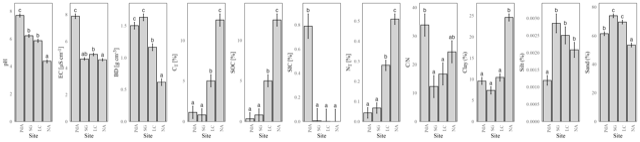
\includegraphics[width=1\textwidth]{img/baseline_by_site.png}
    % The caption remains the same
    \caption{Soil physical and chemical properties across the four study sites (PdA: Pan de Azúcar, SG: Santa Gracia, LC: La Campana, and NA: Nahuelbuta). Letter-based display accompanying soil properties with significant effect for site. Different letters indicate statistically significant differences ($p < 0.05$, Šidák correction).}
    % The label remains the same
    \label{fig:baseline_site}
\end{sidewaysfigure}

\FloatBarrier

\subsection{Biocrust-induced changes in soil properties}
\label{sec:BicorustInducedSoil}

Biocrust presence significantly ($p < 0.05$) influenced several soil properties (Figure \ref{fig:baseline_biocrust_interaction}a), often interacting with the climatic site (Figure \ref{fig:baseline_biocrust_interaction}b). A significant site $\times$ biocrust interaction was observed for bulk density, with biocrusts associated with a decrease in BD in arid PdA but an increase in Mediterranean LC. Biocrust presence significantly affected soil texture overall, associated with a slight decrease in clay and an increase in silt content when averaged across sites. However, the site $\times$ biocrust interaction was significant for clay, showing a notable increase under biocrusts specifically in PdA. Across all sites, biocrust presence led to a small but statistically significant decrease in soil pH, potentially reflecting localized acidification due to respiration \citep{Bachar2010}. C\textsubscript{T} and SOC contents were significantly lower under biocrusts when averaged across all sites. A significant site $\times$ biocrust interaction affected N\textsubscript{T}, showing significantly lower values under biocrusts only in the humid LC and NA sites. The C/N ratio was significantly lower under biocrusts overall, driven partly by changes in PdA. Electrical conductivity (EC) was extremely high in PdA compared to other sites, and the site $\times$ biocrust interaction showed a significant reduction in EC under biocrusts only in PdA.

% I will include it sideways for better visualization
\begin{sidewaysfigure}
    \centering
    % The \includegraphics command remains the same
    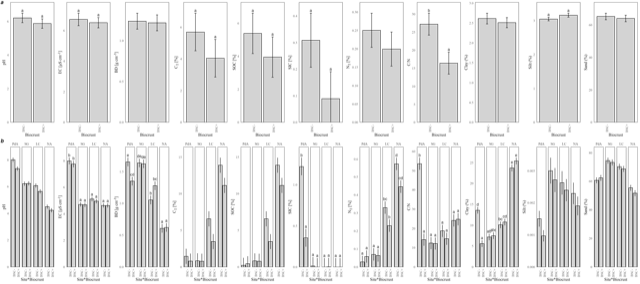
\includegraphics[width=1\textwidth]{img/baseline_by_biocrust_interaction.png}
    % The caption remains the same, clean up the p<0.05 part
    \caption{Biocrust (a) and interaction (b) effects on soil properties. Soil physical and chemical properties across for biocrust (BSC+ vs. BSC-) and the interaction with the site (PdA: Pan de Azúcar, SG: Santa Gracia, LC: La Campana, and NA: Nahuelbuta). Letter-based display accompanying soil properties with significant effect for site or site*biocrust. Different letters indicate statistically significant differences ($p < 0.05$, Šidák correction).} % Use math mode for p < 0.05
    % The label remains the same
    \label{fig:baseline_biocrust_interaction}
\end{sidewaysfigure} % *** End sidewaysfigure environment ***

\FloatBarrier

\subsection{Biocrust and climate interactions on aggregate stability}
\label{sec:BiocrusClimateInducedSoil}

Soil aggregate stability showed clear responses to both the climatic gradient and biocrust cover, particularly when assessed under wet conditions. Overall aggregate stability, indicated by the difference in geometric mean diameter ($\Delta$GMD), significantly increased (lower $\Delta$GMD indicates higher stability) along the climatic gradient from PdA (mean $\Delta$GMD \SI{1.86}{\milli\meter}) to NA (mean $\Delta$GMD \SI{0.83}{\milli\meter}), although SG showed higher stability (mean $\Delta$GMD \SI{1.2}{\milli\meter}) than LC (mean $\Delta$GMD \SI{1.4}{\milli\meter}). The water stability aggregate ratio (WSAR) confirmed this trend, with NA (mean WSAR 81.1\%) being significantly more stable than the other sites (mean WSAR 57.7\% - 73.4\%).

Biocrusts exerted a significant stabilizing effect, particularly on larger aggregates under wet sieving conditions. The presence of biocrusts significantly increased the proportion of water-stable aggregates $>$\SI{2}{\milli\meter} overall. Specifically, the interaction between site and biocrust was significant for wet aggregates in the \SIrange[range-phrase=--,range-units=single]{9.5}{30.0}{\milli\meter} range, showing a stabilizing effect (increase in proportion) in PdA, SG, and LC, but not in the humid NA site. This suggests a threshold effect, where the stabilizing role of biocrusts diminishes as vascular vegetation and associated stabilizing agents become more dominant under humid conditions. Correspondingly, biocrust presence significantly decreased the proportion of water-stable aggregates $<$\SI{2}{\milli\meter} (R\textsubscript{$<$\SI{2}{\milli\meter}}) overall (from mean 63.7\% without biocrusts to 57.5\% with biocrusts) (Figure \ref{fig:aggregate-stability}).

These findings highlight that biocrusts contribute to soil structure by binding particles and microaggregates, likely through mechanisms involving fungal hyphae, cyanobacterial filaments, and the production of extracellular polymeric substances \citep{Six2004,Totsche2018}. While biocrusts influenced bulk C and N contents, the lack of a direct correlation between these bulk changes and stability across all sites suggests that the specific composition and micro-spatial arrangement of organic binding agents within aggregates, rather than just total C or N, are critical for stability \citep{Wagner2007}. The results emphasize the crucial role of biocrusts as primary stabilizing agents in arid and semi-arid ecosystems \citep{BelnapBudel2016}, with their influence gradually yielding to vascular plants and associated soil organic matter dynamics in more humid environments.

\begin{figure}[h!]
	\centering
	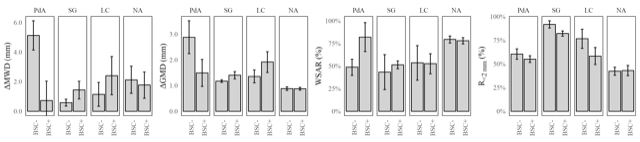
\includegraphics[width=1\textwidth]{img/aggregate stability indexes_se.png}
	\caption{Aggregate stability indexes for Pan de Azúcar (PdA), Santa Gracia (SG), La Campana (LC), and Nahuelbuta (NA) for biocrust (BSC+) and non-biocrust (BSC-) treatments displayes as mean and standard error. $\Delta$MWD: difference in mean weight diameter, $\Delta$GMD: difference in geometric mean diameter, WSAR: water stability aggregate ratio, R$_{<\SI{2}{\milli\meter}}$: ratio of aggregates less than \SI{2}{\milli\meter}.}
	\label{fig:aggregate-stability}
\end{figure}
\FloatBarrier


\section[Effect of biocrust on water flow, erosion and nutrient flow]{Effect of biocrust on water flow, erosion and nutrient flow (manuscript 2)}
\label{sec:BiocrustOnFlows}

This study investigated the role of biological soil crusts (biocrusts) as climate-dependent regulators of erosion, water, and nutrient cycling using rainfall simulation experiments across a 910 km climate gradient in the Coastal Mountain Range of Chile. Four study sites represented coastal semi-arid (SG), inland semi-arid (QdT), Mediterranean (LC), and humid (NA) climates. These sites, characterized by comparable topography and granitic parent material, allowed for assessing biocrust influence under varying climatic conditions by comparing undisturbed soil monoliths with (+) and without (-) biocrust cover. We analyzed surface runoff, percolation flow, sediment transport, and associated carbon (C) and nitrogen (N) fluxes.

Soil properties varied across the climate gradient, reflecting differing weathering intensities and soil development stages relevant to hydrological and erosion responses. Notably, the inland semi-arid site (QdT) exhibited high biocrust cover despite lower water availability compared to the coastal SG site, likely due to protection from disturbance within a fenced area since 2011, fostering biocrust development \citep{Budel2016}. Soil texture across sites was predominantly sandy loam, with clay content increasing southward, influencing water retention and infiltration pathways.

\subsection{Biocrust influence on water flow and sediment transport}
\label{sec:BiocrustOnWaterSesimentsFlows}

Biocrusts significantly modulated water flow and erosion dynamics, though their effects varied with climate and the specific pathway (runoff vs. percolation). Regarding runoff dynamics (Table \ref{tab:runoff_fluxes}), biocrusts delayed runoff initiation across all sites, with a mean delay of 97.7\%. This effect was particularly noticeable at the humid NA site, where dense bryophyte cover increased surface roughness and water storage \citep{Kidron2022}. Overall, biocrusts reduced total runoff volume by an average of 28.0\%, although this was site-specific, ranging from a 72.4\% reduction in NA to an unexpected 36.4\% increase in LC. Despite these impacts on surface flow, biocrusts did not measurably affect the time required for percolation to commence (Table \ref{tab:percolation_fluxes}). The reduction in runoff volume (Table \ref{tab:runoff_fluxes}) coupled with unchanged percolation timing (Table \ref{tab:percolation_fluxes}) indicated enhanced cumulative infiltration and saturated hydraulic conductivity in the presence of biocrusts compared to bare soil. In terms of erosion and sediment flux, biocrusts proved highly effective at reducing soil erosion via surface runoff, decreasing total sediment transport by an average of 69.9\% and sediment concentration in runoff by 60.9\% (Table \ref{tab:runoff_fluxes}). The most significant reduction occurred at the inland semi-arid QdT site, highlighting the protective role of biocrusts  \citep{RodriguezCaballero2018}. Conversely, sediment mobilization via percolation increased by 28.3\%, and sediment concentration in percolation rose by 58.3\% when biocrusts were present. This demonstrates a clear shift in sediment transport dynamics, moving from predominantly surface erosion on bare soil to increased subsurface transport under biocrust cover.

\begin{sidewaystable} % Using sidewaystable instead of table
    % \centering % Centering is often implicit/less relevant for full-page sideways tables
    \begin{threeparttable}
        \caption{Surface runoff fluxes on the study sites (SG: Santa Gracia, QdT: Quebrada de Talca, LC: La Campana, NA: Nahuelbuta) with (+) and without (-) biocrust (BSC) cover. Values correspond to mean $\pm$ standard deviation (SD) of five field replicates. Different letters indicate statistically significant different values based on Šidák correction post-hoc test results.}
        \label{tab:runoff_fluxes}

        % Define column widths/types. S columns align numbers. 'l' for text.
        % Determine table-format based on max digits before/after decimal, plus uncertainty.
        \begin{tabular}{@{} ll S[table-format=3.1(3.1)] l % Time
                             S[table-format=2.0(2.0)] l % Runoff
                             S[table-format=3.0(3.0)] l % Sediment
                             S[table-format=2.1(2.1)] l % Sed. Load
                       @{}}
            \toprule
            % --- Headers ---
            % Using \makecell for multi-line headers with units
            \multicolumn{2}{@{}l}{\textbf{Factor}} % Span first two columns for header alignment
            & \multicolumn{2}{c}{\makecell{\textbf{Time to start runoff}\tnote{a}\\ {[\si{\second}]}}}
            & \multicolumn{2}{c}{\makecell{\textbf{Runoff}\tnote{a}\\ {[\si{\liter\per\hour}]}}}
            & \multicolumn{2}{c}{\makecell{\textbf{Sediment in runoff}\tnote{a}\\ {[\si{\gram\per\meter\squared\per\hour}]}}}
            & \multicolumn{2}{c}{\makecell{\textbf{Sediment load of runoff}\tnote{a}\\ {[\si{\gram\per\liter\per\meter\squared}]}}} \\
            \cmidrule(lr){3-4} \cmidrule(lr){5-6} \cmidrule(lr){7-8} \cmidrule(lr){9-10} % Rules under spanned headers

            % --- Data Rows ---
            % Mean Site Effects
            Mean $\pm$ SD & SG   & 65.1 \pm 20.7  & (a) & 49 \pm 18  & (b) & 617 \pm 473 & (c) & 12.1 \pm 7.9  & (a) \\
                          & QdT  & 78.7 \pm 30.4  & (a) & 40 \pm 16  & (a) & 398 \pm 459 & (b) & 9.6 \pm 9.6   & (a) \\
                          & LC   & 83.5 \pm 56.0  & (a) & 39 \pm 22  & (a) & 241 \pm 293 & (b) & 7.3 \pm 8.8   & (a) \\
                          & NA   & 236.7 \pm 273.0& (b) & 44 \pm 43  & (a) & 28 \pm 44   & (a) & 3.0 \pm 14.0  & (a) \\
            \midrule
            % Mean Biocrust Effects
            Biocrust      & BSC+ & 154.0 \pm 211.5& (b) & 36 \pm 21  & (a) & 149 \pm 222 & (a) & 4.5 \pm 10.4  & (a) \\
                          & BSC- & 77.9 \pm 33.8  & (a) & 50 \pm 31  & (b) & 495 \pm 492 & (b) & 11.5 \pm 10.0 & (b) \\
            \midrule
            % Interaction Effects
            Site*Biocrust & SG BSC+ & 62.7 \pm 21.2 & (ab) & 44 \pm 16 & (ab) & 340 \pm 340 & (bc)  & 7.5 \pm 5.7  & (abc)  \\
                          & SG BSC- & 67.5 \pm 20.6 & (ab) & 54 \pm 18 & (ab) & 873 \pm 456 & (d)   & 16.7 \pm 7.1 & (de)   \\ \addlinespace
                          & QdT BSC+& 87.3 \pm 37.5 & (ab) & 38 \pm 15 & (ab) & 131 \pm 96  & (ab)  & 3.3 \pm 2.0  & (abd)  \\
                          & QdT BSC-& 70.1 \pm 18.7 & (ab) & 42 \pm 18 & (ab) & 665 \pm 524 & (cd)  & 15.8 \pm 10.2& (ce)   \\ \addlinespace
                          & LC BSC+ & 85.8 \pm 67.1 & (ab) & 45 \pm 20 & (ab) & 87 \pm 94   & (a)   & 2.1 \pm 1.9  & (a)    \\
                          & LC BSC- & 81.2 \pm 44.6 & (ab) & 33 \pm 23 & (ab) & 395 \pm 344 & (bc)  & 12.6 \pm 9.9 & (bcde) \\ \addlinespace
                          & NA BSC+ & 380.4 \pm 329.5& (b) & 19 \pm 23 & (a)  & 16 \pm 49   & (a)   & 5.2 \pm 19.9 & (abcde)\\
                          & NA BSC- & 93.0 \pm 40.2 & (a) & 69 \pm 45 & (b)  & 40 \pm 36   & (a)   & 0.9 \pm 1.2  & (abcde)\\
            \bottomrule
        \end{tabular}

        % --- Table Notes ---
        \begin{tablenotes}[para,flushleft] % para puts notes on one line if space, flushleft aligns note markers
           \item[a] Letter-based display accompanying surface runoff parameters. Different letters within a column section (Mean, Biocrust, or Site*Biocrust interaction) indicate statistically significant differences ($p < 0.05$, Šidák correction).
        \end{tablenotes}

    \end{threeparttable}
\end{sidewaystable} % *** End the sidewaystable environment ***


\begin{sidewaystable} % Using sidewaystable for landscape orientation
    \begin{threeparttable}
        \caption{Percolating water fluxes on the study sites (SG: Santa Gracia, QdT: Quebrada de Talca, LC: La Campana, NA: Nahuelbuta) with (+) and without (-) biocrust (BSC) cover. Values correspond to mean $\pm$ standard deviation (SD) of five field replicates. Different letters indicate statistically significant different values based on Šidák correction post-hoc test results.}
        \label{tab:percolation_fluxes} % Unique label for this table

        % Use tabular* to fill the linewidth.
        % Column structure MUST match Table 2: ll Sl Sl Sl Sl
        % Add 'l' columns even where no letters exist in Table 3.
        \begin{tabular*}{\linewidth}{@{\extracolsep{\fill}} % Distribute extra space
                             ll % Factor Column 1 & 2 (left aligned)
                             @{\extracolsep{\fill}} % Space after Factor columns
                             S[table-format=3.0(3.1)] l % Time Column 3 (S) + EMPTY Letter Column 4 (l)
                             @{\extracolsep{\fill}} % Space after Time group
                             S[table-format=2.1(2.0)] l % Percolation Column 5 (S) + Letter Column 6 (l)
                             @{\extracolsep{\fill}} % Space after Percolation group
                             S[table-format=2.0(2.0)] l % Sediments Column 7 (S) + Letter Column 8 (l)
                             @{\extracolsep{\fill}} % Space after Sediments group
                             S[table-format=1.1(2.1)] l % Sed. Load Column 9 (S) + EMPTY Letter Column 10 (l)
                             @{} % No padding at the end
                             }
            \toprule
            % --- Headers ---
            % Span 2 columns (S+l) for EACH parameter header for consistent layout
            \multicolumn{2}{@{}l}{\textbf{Factor}}
            & \multicolumn{2}{c}{\makecell{\textbf{Time to start}\\\textbf{percolation flow}\\ {[\si{\second}]}}}
            & \multicolumn{2}{c}{\makecell{\textbf{Percolation}\tnote{a}\\ {[\si{\liter\per\hour}]}}}
            & \multicolumn{2}{c}{\makecell{\textbf{Sediments in}\\\textbf{percolation flow}\tnote{a}\\ {[\si{\gram\per\meter\squared\per\hour}]}}}
            & \multicolumn{2}{c}{\makecell{\textbf{Sediment load in}\\\textbf{percolation}\\ {[\si{\gram\per\liter\per\meter\squared}]}}} \\
            % cmidrules span 2 cols each, matching headers
             \cmidrule(lr){3-4} \cmidrule(lr){5-6} \cmidrule(lr){7-8} \cmidrule(lr){9-10}

            % --- Data Rows ---
            Mean $\pm$ SD & SG   & \num{223 \pm 190}   &     & \num{18.0 \pm 14}  & (a) & \num{19 \pm 34} &     & \num{4.2 \pm 19.7} &   \\
                          & QdT  & \num{175.0 \pm 94.5}&     & \num{22.8 \pm 15}  & (a) & \num{7 \pm 10}  &     & \num{0.2 \pm 0.3}  &   \\
                          & LC   & \num{234 \pm 183}   &     & \num{22.4 \pm 13}  & (a) & \num{13 \pm 15} &     & \num{0.5 \pm 0.5}  &   \\
                          & NA   & \num{145 \pm 169}   &     & \num{65.0 \pm 39}  & (b) & \num{23 \pm 25} &     & \num{0.4 \pm 0.4}  &   \\
            \midrule
            Biocrust      & BSC+ & \num{171 \pm 133}   &     & \num{42.6 \pm 34}  & (b) & \num{19 \pm 22} & (b) & \num{0.5 \pm 0.5}  &   \\
                          & BSC- & \num{218 \pm 190}   &     & \num{21.5 \pm 21}  & (a) & \num{12 \pm 24} & (a) & \num{2.1 \pm 13.7} &   \\
            \midrule
            Site*Biocrust & SG BSC+  & \num{202 \pm 103}   &     & \num{24.8 \pm 15}  & (ab) & \num{19 \pm 18} &     & \num{0.7 \pm 0.5}  &   \\
                          & SG BSC-  & \num{244 \pm 251}   &     & \num{11.1 \pm 10}  & (a)  & \num{18 \pm 46} &     & \num{7.5 \pm 27.5} &   \\ \addlinespace
                          & QdT BSC+ & \num{148.0 \pm 63.9}&     & \num{30.5 \pm 13}  & (b)  & \num{9 \pm 13}  &     & \num{0.3 \pm 0.3}  &   \\
                          & QdT BSC-& \num{202 \pm 113}   &     & \num{15.1 \pm 13}  & (ab) & \num{5 \pm 6}   &     & \num{0.2 \pm 0.2}  &   \\ \addlinespace
                          & LC BSC+  & \num{226 \pm 223}   &     & \num{23.5 \pm 14}  & (ab) & \num{17 \pm 19} &     & \num{0.6 \pm 0.5}  &   \\
                          & LC BSC-  & \num{241 \pm 139}   &     & \num{21.3 \pm 14}  & (ab) & \num{9 \pm 9}   &     & \num{0.4 \pm 0.3}  &   \\ \addlinespace
                          & NA BSC+  & \num{107.0 \pm 35.6}&     & \num{91.5 \pm 28}  & (c)  & \num{30 \pm 32} &     & \num{0.4 \pm 0.4}  &   \\
                          & NA BSC-  & \num{183 \pm 234}   &     & \num{38.5 \pm 30}  & (b)  & \num{16 \pm 15} &     & \num{0.4 \pm 0.3}  &   \\

            \bottomrule
        \end{tabular*} % End tabular*

        % --- Table Notes ---
        \begin{tablenotes}[para,flushleft]
           \item[a] Letter-based display accompanying parameters where shown. Different letters within a column section (Mean, Biocrust, or Site*Biocrust interaction) indicate statistically significant differences ($p < 0.05$, Šidák correction).
        \end{tablenotes}

    \end{threeparttable}
\end{sidewaystable} % End the sidewaystable environment

\FloatBarrier

\FloatBarrier

\subsection{Biocrust modulation of carbon and nitrogen fluxes}
\label{sec:BiocrustOnNutrientFlows}

Biocrusts significantly altered the transport pathways and amounts of C and N in both sediment-bound and dissolved forms, with effects dependent on climate and site conditions (Figure \ref{fig:nutrient-flow}). For carbon fluxes, sediment-associated C loss via runoff generally increased with climatic humidity. Biocrusts significantly reduced this sediment C loss, by up to a factor of four compared to bare soil. In percolation flow, biocrusts also reduced the C content in mobilized sediments, an effect most pronounced in drier climates where reductions reached 20-40\%. Furthermore, biocrusts consistently increased dissolved organic carbon (DOC) concentrations in runoff across all sites, suggesting an alteration of C cycling pathways towards leaching rather than just physical erosion \citep{Baumert2021}. Similar patterns, though moderated by site*biocrust interactions, were observed for DOC transported via percolation. Regarding nitrogen fluxes, sediment-associated N loss via runoff also increased with humidity. The biocrust effect on this sediment N was strongly site-specific, causing an increase in SG but a decrease in NA, and explaining 48.8\% of the observed variability. Dissolved organic nitrogen (DON) fluxes in runoff showed trends analogous to DOC, generally increasing with biocrust presence, especially in northern sites like SG (increasing from 1.3$\pm$1.0 ppm in BSC- to 2.2$\pm$2.0 ppm in BSC+). However, a contrasting effect was observed at the humid NA site, where biocrusts decreased DON in runoff (from 0.6$\pm$0.7 ppm in BSC- to 0.3$\pm$0.8 ppm in BSC+), potentially indicating enhanced N immobilization or uptake in this N-richer ecosystem. DON fluxes transported via percolation followed similar site-dependent trends influenced by biocrust interactions.

\begin{figure}[h!]
	\centering
	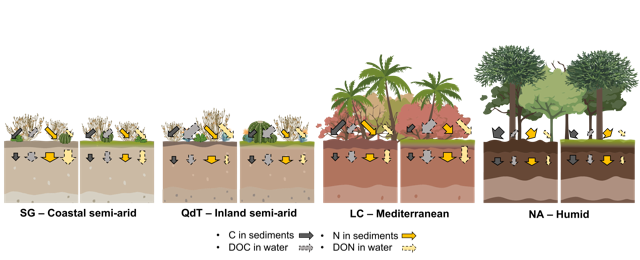
\includegraphics[width=1\textwidth]{img/nutrient-flow-diagram.png}
	\caption{Representation of total carbon in sediments and DOC in water fluxes for the four study sites. The diagrams at the right side with slightly green surface represents the BSC+ treatments and the one at the left the BSC-. Grey-filled arrows correspond to C fluxes, and yellowish arrows to N. At the same time, arrows with solid borders correspond to the flow attached to the sediments, and dashed arrows dissolved in water. Each type of arrow is proportional inside each group in width to the concentration of nutrients and in length to the mass of it.}
	\label{fig:nutrient-flow}
\end{figure}

\FloatBarrier

Overall, biocrusts play a crucial, climate-dependent role in regulating water flow, significantly reducing surface runoff erosion, but potentially increasing subsurface sediment transport. They profoundly influence C and N cycling, generally reducing C losses via runoff while altering dissolved nutrient pathways, with specific effects on N mobilization varying strongly between arid and humid environments.

\section[Microbial, plant and moisture controls on soil structure and functionality]{Microbial, plant and moisture controls on soil structure and functionality (manuscripts 3, 4 and 5)}
\label{sec:MicrobesPlantsMoistureStructure}

Beyond the direct impacts of biological soil crusts (BSCs) and the broad climatic gradient, further investigations using subsets of the study sites (primarily arid Pan de Azúcar (PdA) and semi-arid Santa Gracia (SG), but also including mediterranean La Campana (LC) and humid Nahuelbuta (NA) in Manuscript 4) provided deeper insights into the roles of the indigenous microbial community, plant roots, and moisture dynamics in shaping soil aggregation, organic matter turnover, and nutrient cycling. These studies employed controlled laboratory incubations simulating specific scenarios: a shift to humid conditions for arid/semi-arid soils (Manuscript 3), repeated wetting-drying (W-D) versus constant moisture (CM) regimes across the climate gradient (Manuscript 4), and the natural transition from a living rhizosphere to a decomposing detritusphere in semi-arid soil (Manuscript 5).

A central finding emerging from these experiments is that the impact of microbial activity on soil aggregation and related properties is highly dependent on the origin of the soil and the prevailing environmental conditions. This was clearly demonstrated in the moisture regime experiment (Manuscript 4), where the responses of native, microbially active soils to repeated wetting-drying (W-D) cycles were compared against sterilized controls across the climate gradient. Principal Component Analysis visually distinguished the trajectories of native versus sterile soils under W-D stress, directly highlighting the significant contribution of microbial activity to changes in soil edaphic properties (Figure \ref{fig:PCA-microbes}). Crucially, the nature of this microbial influence differed markedly between climate zones. In arid soils, the microbially-influenced samples were primarily characterized by changes in aggregate C/N ratios, suggesting accelerated turnover of labile organic matter (OM) fueled by the Birch effect (Figure \ref{fig:PCA-microbes}A). In contrast, microbially-influenced semi-arid and mediterranean soils under W-D were distinguished from controls mainly by shifts in aggregate size distribution, particularly an increase in microaggregates (MIC) relative to macroaggregates (MAC) (Figure \ref{fig:PCA-microbes}B-C). This direct comparison underscores that while microbes actively mediate soil structural changes during moisture fluctuations, the specific mechanisms and outcomes (OM turnover vs. aggregate reorganization) are strongly dictated by the climate legacy imprinted on the soil and its microbial community.

\begin{figure}[h!]
	\centering
	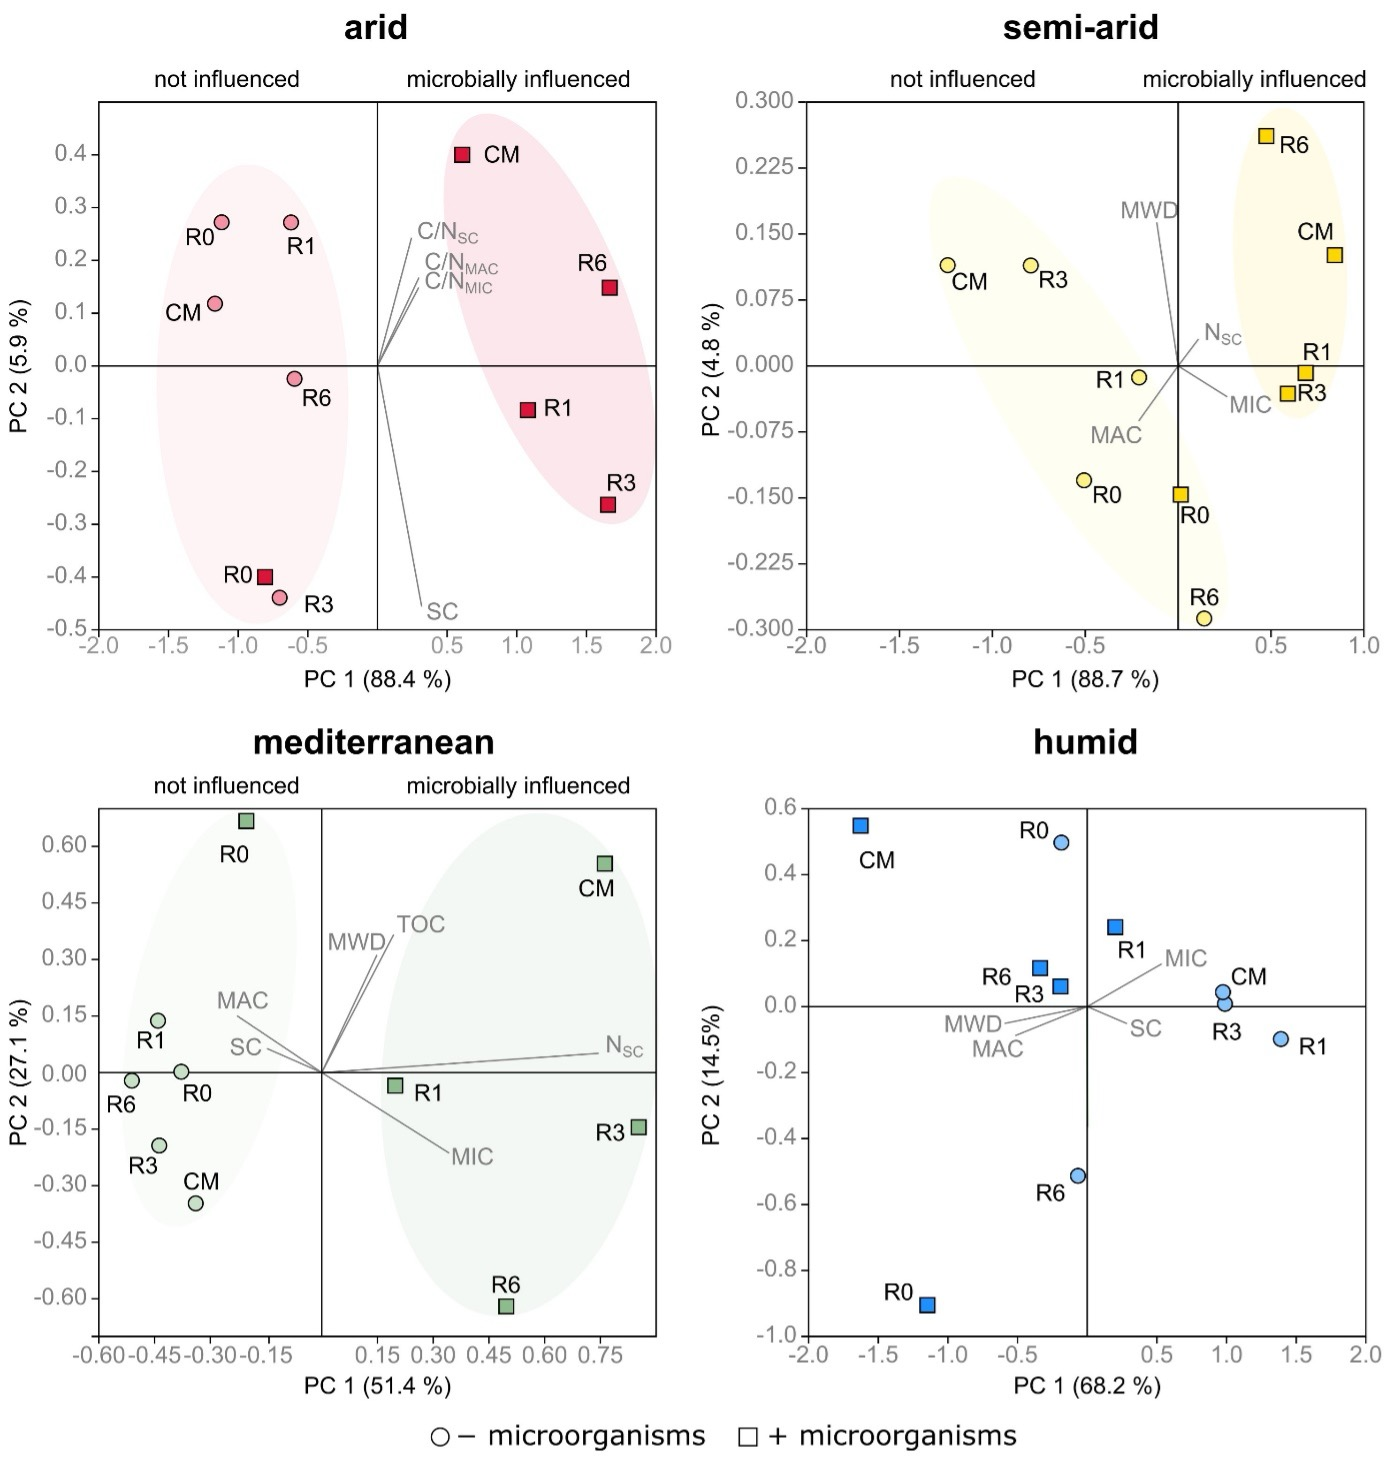
\includegraphics[width=1\textwidth]{img/PCA-microbes-structure.jpg}
	\caption{Principal Component Analyses of soil properties in native soils (squares) and sterilized soils (circles) including significant soil properties. A) arid, B) semi-arid, C) mediterranean and D) humid site. Microbial influence is indicated by sample separation along the x-axis.}
	\label{fig:PCA-microbes}
\end{figure}

\FloatBarrier

Further results support this picture of context-dependent microbial influence and climate legacy effects. The observed increase in aggregate C/N ratios in microbially active arid soils (Figure \ref{fig:bacterial-abundance}A) aligns with findings of stimulated microbial abundance under W-D but also a net breakdown of MAC and only a slight decrease in overall aggregate stability (MWD) (Manuscript 4), consistent with rapid consumption of labile OM released from decomposing larger aggregates. The microaggregate formation observed in microbially influenced semi-arid and mediterranean soils (Figure \ref{fig:PCA-microbes}B-C) corresponds with outcomes where overall stability either slightly decreased (semi-arid) or increased (mediterranean) (Manuscript 4), suggesting different stabilization pathways potentially involving OM redistribution or transformation.

\begin{figure}[h!]
	\centering
	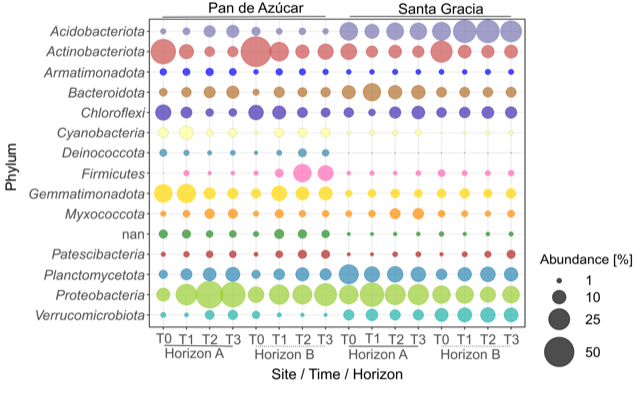
\includegraphics[width=1\textwidth]{img/bacterial-abundance.png}
	\caption{Relative abundance of top 15 bacterial phyla for Pan de Azúcar and Santa Gracia and the different time points. Time is represented as T0 (original), T1 (2 weeks), T2 (12 weeks) and T3 (16 weeks). Each bubble is the mean of the different treatments (in situ, BSCs and plants) and technical triplicates.}
	\label{fig:bacterial-abundance}
\end{figure}

\FloatBarrier

The importance of climate legacy was also evident in the differential resilience of microbial communities themselves. The arid PdA community, adapted to stable hyperaridity, showed significant structural changes and diversity loss under simulated humid conditions (Manuscript 3), while the semi-arid SG community, from a more variable climate, demonstrated greater stability (Figure \ref{fig:bacterial-abundance}), mirroring the patterns observed in the PCA analysis (Figure \ref{fig:PCA-microbes}).

Beyond the intrinsic microbial community and moisture effects, the powerful role of plants was confirmed (Manuscript 5). Living roots acted as potent drivers of macroaggregation in both topsoil and subsoil of semi-arid origin. However, a distinct root legacy effect was apparent, as this enhanced aggregation only persisted after plant death in the topsoil, indicating a requirement for continuous C input or greater inherent stability factors in the subsoil. This transition from rhizosphere to detritusphere also drove a microbial succession from fungal to Gram-positive bacterial dominance and altered OM protection mechanisms, notably increasing occluded POM in the topsoil detritusphere.

\chapter{Conclusion \& Outlook}

This research investigated the multifaceted role of biological soil crusts (biocrusts) and microbial communities in shaping soil development, stability, and nutrient cycling across a climate gradient in the Chilean Coastal Range. By combining field observations, laboratory experiments, and advanced analytical techniques, this work provides valuable insights into the complex interactions between biota, climate, and soil processes.

A key focus of this research was to understand the influence of biocrusts on soil aggregate stability and their interplay with soil properties along a climate gradient. Four sites representing arid, semi-arid, Mediterranean, and humid conditions were selected, allowing for a comparative analysis of biocrust effects under contrasting environmental conditions. The results revealed significant variations in soil properties along the gradient, with bulk density decreasing and soil organic carbon (SOC), total nitrogen (N\textsubscript{T}), and clay content increasing with humidity. These variations reflect the influence of climate on weathering processes, organic matter accumulation, and soil development \cite{Jenny1941}. Biocrust cover significantly influenced soil properties, particularly in arid and semi-arid sites, where it increased SOC and N\textsubscript{T} content and altered soil texture, indicating its role in trapping organic matter and modifying soil structure \citep{Belnap2003,Bowker2006}. Aggregate stability, a key indicator of soil resilience to erosion, was enhanced by the presence of biocrusts across all climates, with the most pronounced effect observed in the arid site. This finding underscores the crucial role of biocrusts in protecting vulnerable soils in dryland environments \citep{Chamizo2012}. The difference in geometric mean diameter of aggregates further emphasized the stabilizing effect of biocrusts, particularly in the arid site, where they significantly increased aggregate size.

Extending the investigation of biocrusts beyond their impact on soil structure, this research also explored their role as climate-dependent regulators of erosion, water, and nutrient cycling. Utilizing rainfall simulation experiments across the same climate gradient, the study assessed the effects of biocrusts on surface runoff, percolation flow, and sediment and nutrient fluxes. Biocrusts significantly delayed the initiation of runoff and reduced overall runoff volume in all climates, highlighting their capacity to retain water and mitigate erosion \citep{Kidron2022}. The influence of biocrusts on sediment discharge was equally pronounced, with significant reductions observed across all sites, particularly in the inland semi-arid environment. Furthermore, biocrusts influenced both sediment-bound and dissolved carbon and nitrogen dynamics, with contrasting effects observed across the climate gradient. While biocrusts increased carbon content in sediments mobilized by runoff at drier sites, they also enhanced dissolved organic carbon (DOC) concentrations, indicating alterations in carbon cycling pathways. Similarly, biocrusts influenced nitrogen fluxes, increasing dissolved organic nitrogen (DON) concentrations, but with varying effects across the climatic gradient. These findings underscore the complex and context-dependent role of biocrusts in regulating both hydrological and biogeochemical processes in soil ecosystems.

Complementing the field and rainfall simulation studies, laboratory experiments explored the microbial drivers of soil aggregate turnover across different climates and moisture regimes. By subjecting soils from the same climate gradient sites to controlled wetting-drying (W-D) cycles, this research aimed to dissect the relative contributions of abiotic and biotic factors in shaping soil structure. The results revealed distinct patterns in aggregate size distribution and stability across climates and in response to W-D cycles. Sterilization significantly altered aggregate dynamics, highlighting the crucial role of microbial communities in soil structure formation and stabilization \citep{Six2004}. Microbial abundance, diversity, and community composition also exhibited climate-specific responses to W-D cycles, reflecting the adaptive strategies of soil microorganisms to fluctuating moisture conditions. W-D cycles also impacted predicted microbial functions, influencing the decomposition of organic matter and nutrient cycling processes.

Building upon the findings related to microbial influence on soil aggregate dynamics, the research further explored the role of microbial communities in initial soil formation under simulated climate change scenarios. Using soil samples from arid and semi-arid sites, the study simulated increased humidity conditions, reflecting potential climate change projections for these regions. The results revealed significant shifts in microbial community structure and function in response to the simulated climate change, with certain microbial groups, notably Sphingomonas, exhibiting increased abundance and potential for nitrogen fixation. These findings underscore the importance of soil legacy effects and the potential for microbial communities to adapt and mediate soil processes under changing environmental conditions.

Lastly, the research delved into the specific role of roots in regulating soil aggregation and organic matter dynamics, focusing on the transition from rhizosphere to detritusphere. Microcosm experiments with living and decaying cereal roots revealed significant differences in soil aggregate formation, microbial community composition, and organic matter characteristics. Living roots promoted the development of macroaggregates, particularly in the subsoil, while decaying roots stimulated microbial activity and altered organic matter decomposition pathways. These findings emphasize the dynamic interplay between living and decaying roots and their influence on soil structure, microbial communities, and organic matter cycling. The transition from rhizosphere to detritusphere represents a shift from root-driven soil formation to decomposition-dominated processes, highlighting the interconnectedness of plant and microbial contributions to soil ecosystem functioning.

In summary, this body of research demonstrates the complex and interconnected roles of biocrusts, microbial communities, and plant roots in shaping soil development, stability, and nutrient cycling across a climate gradient. Biocrusts act as key regulators of surface processes, enhancing soil aggregate stability, reducing erosion, and modulating water and nutrient fluxes. Microbial communities, as the engines of biogeochemical processes, drive soil aggregation, organic matter decomposition, and respond dynamically to changes in moisture availability and climate conditions. Plant roots, both living and decaying, influence soil structure formation, microbial communities, and organic matter dynamics, with distinct effects observed in rhizosphere and detritusphere environments.

Future research should focus on further disentangling the complex interactions between biocrusts, microbial communities, and plants. This includes investigating the specific mechanisms driving biocrust formation and their influence on different soil types, exploring the functional diversity of microbial communities involved in soil aggregate formation, and examining the long-term legacy effects of plant-soil interactions on soil carbon sequestration. Moreover, considering the projected impacts of climate change, future studies should assess the resilience of biocrusts and microbial communities to altered precipitation patterns, temperature regimes, and increased atmospheric $CO_2$ concentrations. By deepening our understanding of these complex interactions, we can develop more effective strategies for soil conservation, ecosystem management, and promoting the sustainable use of soil resources in the face of global environmental change.


% --- Bibliography ---
\bibliographystyle{apalike} % Or other natbib style
\bibliography{literatur}

\appendix

% --- Appendices ---
% --- Custom Appendix Overview Page ---
% Adds "Appendix" to the Table of Contents
\addcontentsline{toc}{chapter}{Appendix}
% Creates an unnumbered chapter heading for the list
\chapter*{Appendix}
\label{chap:appendix_overview} % Label for reference if needed

% --- List of Manuscripts (Manual Entry) ---
% This section manually lists the manuscripts like in your example.
% You will need to MANUALLY UPDATE THE PAGE RANGES (pp. X - Y)
% after compiling the document fully at least twice.

\noindent % Prevents paragraph indentation
\textbf{Manuscript 1} \hfill \textbf{pp. 59 - 72} \\ % <-- UPDATE PAGE NUMBERS MANUALLY
GALL, C.; OHAN, J.; GLASER, K.; KARSTEN, U.; SCHLOTER, M.; SCHOLTEN, T.; SCHULZ, S.; SEITZ, S. \& KURTH, J. K. (2022): \\
\textit{Biocrusts: Overlooked hotspots of managed soils in mesic environments.} \\
Journal of Plant Nutrition and Soil Science, 185 (6), 745-751. DOI: 10.1002/jpln.202200252.

\vspace{\baselineskip} % Adds a line space between entries

\noindent
\textbf{Manuscript 2} \hfill \textbf{pp. 73 - 111} \\ % <-- UPDATE PAGE NUMBERS MANUALLY
GALL, C.; NEBEL, M.; QUANDT, D.; SCHOLTEN, T. \& SEITZ, S. (2022): \\
\textit{Pioneer biocrust communities prevent soil erosion in temperate forests after disturbances.} \\
Biogeosciences, 19, 3225–3245. DOI: 10.5194/bg-19-3225-2022.

\vspace{\baselineskip}

\noindent
\textbf{Manuscript 3} \hfill \textbf{pp. 112 - 126} \\ % <-- UPDATE PAGE NUMBERS MANUALLY
GALL, C.; NEBEL, M.; SCHOLTEN, T.; THIELEN, S. M. \& SEITZ, S. (in preparation): \\
\textit{On the impact of soil-moss combinations on surface runoff, percolation, soil erosion, and temporal dynamics of soil water content.}

\vspace{\baselineskip}

\noindent
\textbf{Manuscript 4} \hfill \textbf{pp. 127 - 159} \\ % <-- UPDATE PAGE NUMBERS MANUALLY
THIELEN, S. M.; GALL, C.; EBNER, M.; NEBEL, M.; SCHOLTEN, T. \& SEITZ, S. (2021): \\
\textit{Water`s path from moss to soil: A multi-methodological study on water absorption and evaporation of soil moss combinations.} \\
Journal of Hydrology and Hydromechanics, 69 (4), 421-435. DOI: 10.2478/johh-2021-0021.



% Other potential appendix sections:
% \chapter{Abbreviations \& Glossary}

\begin{longtable}[l]{p{.2\textwidth}p{.75\textwidth}}
% \endfirsthead
\endhead
\endfoot
% \endlastfoot
\textit{Bubble} & A structure in the graph topology that is being formed by variable sequence. It is defined as a closed subgraph with an upstream and downstream anchor \textit{node} and a set of \textit{nodes} in between them that represent variable sequence (\autoref{fig:basictube}). A looser formulation of this concept are \textit{snarls} \citep{Paten2018-qj}. \\
\textit{Core} & Part of a \textit{pan-genome} or \textit{pan-proteome} that is shared by all, or a large fraction of the accessions that are part of it \\
\textit{Core level} & A concept used by \textit{panSV} to describe the sharedness of a \textit{node} in the \textit{pan-genome}. The core level is defined as the number of genomes that contain the sequence stored in this \textit{node} and can differ from the number of \textit{paths} that traverse through it, e.g. in the case of a duplication event. \\
\textit{DAG} & Directed Acyclic Graph - A type of graph that prohibits loops in its structure to go back to previous \textit{nodes}. \\ 
\textit{Edge} & Connective feature of a genome graph that orders and connects the \textit{nodes}. \\
\textit{GFA} & Graphical Fragment Assembly - a file format to store graphs in a human readable form \citep{gfa_2021}. \\
\textit{HDR} & Highly Diverged Region - region in a genome that contains a multitude of smaller variants, above the average of the surrounding sequence. As defined by the pairwise variant detection tool SyRI \citep{Goel2019-rx}. \\
\textit{InDel} & Insertion-Deletion variation events in a reference framework that induces the polarity of sequence being inserted, or deleted from it. This term is slowly being replaced by \textit{PAV}. \\
\textit{Mobilome} & Fraction of the genome that consists of mobile elements such as \textit{TEs}. \\
\textit{MUM} & Maximal Unique Match - largest possible unique alignment between sequences \\
\textit{Node} & Element of a genome graph that stores the sequence. \\
\textit{OG} & Orthogroup - Group of orthologous genes. \\
\textit{Path} & Colored traversal through a set of consecutive \textit{nodes}, and \textit{edges} of a graph. A path represents longer sequences in the graph, such as the input genomes. By following it through the graph the full sequence can be recovered. \\
\textit{Pan-genome} & Combined collection of genetic sequence of multiple individuals to represent a larger population. \\
\textit{Pan-proteome} & Collection of genes, or transcripts from multiple individuals that represent an enriched collection and the frequency of their occurrence in a larger population. \\
\textit{PAV} & Presence-Absence variation events. A type of genetic variation where sequence has been gained or lost. \\
\textit{Private} &Part of a \textit{pan-genome} or \textit{pan-proteome} that is shared by no other, or very few other individuals. \\
\textit{Shell} & Part of a \textit{pan-genome} or \textit{pan-proteome} that is niether \textit{core}, nor \textit{private}. \\
\textit{Snarl} & A structure in the graph topology that represents variable sequence in the graph. In contrast to a \textit{bubble} this structure does not have to be a closed subgraph with up- and downstream anchors, but can have additional connections into it, or lack one of the anchors \citep{Paten2018-qj}. \\
\textit{SNP} & Single-Nucleotide-Polymorphism - Variation between two DNA sequences where a single base is replaced by another single base. \\
\textit{Superbubble} & A large substructure of the graph. It follows the definition of a \textit{bubble}, but contains at least one smaller \textit{bubble} inside. \\
\textit{SV} & Structural Variation - Large sequence variation that alters the structure of the genome, for example PAVs, duplications, or translocations. \\
\textit{TE} & Transposable Element - Mobile elements in the DNA sequence that are able to replicate themselves and insert into the genome. \\
\textit{Traversal} & A collection of consecutive \textit{nodes}, and \textit{edges} in a graph that has a defined start and end \textit{node}. 
\end{longtable}


% \include{tex/Glossary}
% \chapter{Supplementary}

\section{Supplementary Figures}

\begin{figure}[h!]
	\centering
	\includegraphics[width=\textwidth]{img/sixRefCoordinates}
	\caption{\textbf{SixRef coordinates} - Geographic locations of the six accessions chosen for assembly.}
	\label{fig:sixRefCoords}
\end{figure}

\begin{figure}[h!]
	\centering
	\includegraphics[width=\textwidth]{img/dotplot}
	\caption{\textbf{Assembly dot-plots} - Synteny representation of the six \textit{de-novo} assemblies, based on \textit{minimap2} alignments with the \textit{TAIR10} reference genome to show the high level of synteny and reveal large scale inversions. Breakpoints are mostly located in the pericentromeric regions, together with a set of inversions.}
	\label{fig:dotplots}
\end{figure}

\begin{figure}[h!]
	\centering
	\includegraphics[width=\textwidth]{img/SyRIrear}
	\caption{\textbf{\textit{SyRI} rearrangements} - Large scale structural rearrangements detected by \textit{SyRI}. The majority of the chromosomes are highly collinear, and differences can mostly be observed in the pericentromeric regions.}
	\label{fig:SyRIrear}
\end{figure}

\begin{figure}[h!]
	\centering
	\includegraphics[width=\textwidth]{img/panSVbubbleCount}
	\caption{\textbf{\textit{panSV} bubbles} - Distribution of core levels of variable regions detected by \textit{panSV}. Most of the regions have core level 7 and only a smaller fraction is nested within them.}
	\label{fig:panSVbubbleCount}
\end{figure}

\begin{figure}[h!]
	\centering
	\includegraphics[width=0.85\textwidth]{img/TEcoverageHeat2}
	\caption{\textbf{TE node coverage} - Heat map of the coverage of nodes ($>$50 bp) that are annotated as containing a TE in at least one accession of the graph.}
	\label{fig:TEcoverageHeat}
\end{figure}

\begin{figure}[h!]
	\centering
	\includegraphics[width=0.85\textwidth]{img/orthogroupPanZscore}
	\caption{\textbf{Orthogroup Z-Score} - Z-Score matrix of the estimated copy numbers of orthogroups, based on the number coverage of the accessions mapped to the graph.}
	\label{fig:orthoPanZ}
\end{figure}

\FloatBarrier

\section{Supplementary Tables}

\begin{table}[h]
	\centering
	\caption{\textbf{Reference based variant calls} - Number and size of reference based variant calls, of the sixRef accessions, in comparison to the \textit{TAIR10} reference genome, made with three different approaches. Short-read based variant calls made as part of the 1001 Genomes Project, pairwise alignment based variants called using \textit{SyRI} from the \textit{de-novo} chromosome scaffolds aligned to the \textit{TAIR10} reference genome, graph based variants, extracted from the graph using \textit{vg deconstruct}. The variants were classified as \textit{SNPs} (one base pair replaced by another base pair), \textit{small variants} ($<$50bp), and \textit{large variants} ($\geq$ 50bp).}
	\resizebox{0.8\textwidth}{!}{
		\begin{tabular}{l|rrrrr}
			& \multicolumn{1}{l}{\# Variants} & \multicolumn{1}{l}{\% Variants} & \multicolumn{1}{l}{Size {[}Mb{]}} & \multicolumn{1}{l}{avg. size} & \multicolumn{1}{l}{median size} \\ \hline
			\multicolumn{6}{c}{Short-read based variants} \\ \hline
			Total & 1,570,148 & 100 & 1.7 & 1.1 & 1 \\
			\textit{SNP} & 1,443,401 & 91.9 & 1.4 & 1 & 1 \\
			\textit{small variant} & 126,747 & 8.1 & 0.2 & 1.8 & 3 \\
			\textit{large variant} & 0 & 0 & 0 & 0 & 0 \\ \hline
			\multicolumn{6}{c}{\textit{Pairwise alignment based variants}} \\ \hline
			Total & 2,589,009 & 100 & 8.2 & 3.2 & 1 \\
			\textit{SNP} & 1,963,863 & 75.9 & 2 & 1 & 1 \\
			\textit{small variant} & 609,648 & 23.6 & 1.5 & 2.5 & 1 \\
			\textit{large variant} & 15,498 & 0.6 & 4.8 & 306.7 & 1 \\ \hline
			\multicolumn{6}{c}{\textit{Graph based variants}} \\ \hline
			Total & 1,869,605 & 1 & 88.6 & 47.4 & 1 \\
			\textit{SNP} & 1,272,633 & 68.1 & 1.3 & 1 & 1 \\
			\textit{small variant} & 539,644 & 0.28.9 & 2.2 & 4 & 2 \\
			\textit{large variant} & 57,328 & 3.1 & 85.2 & 1486.5 & 154
		\end{tabular}
	}
	\label{tab:refGraphCalls}
\end{table}

\begin{table}[h]
	\centering
	\caption{\textbf{Variant call overlap} - Variants that did not intersect with all other sets were overlapped with the remaining variants of the sets. Variants were classified as \textit{small} ($<$50bp) and \textit{large} ($\geq$ 50bp). \textit{SNPs} were excluded.}
	\resizebox{0.8\textwidth}{!}{
		\begin{tabular}{l|rrrrl}
			& \multicolumn{2}{c}{small variants} & \multicolumn{2}{c}{large variants}& \\
			& \multicolumn{1}{l}{\# variants} & \multicolumn{1}{l}{\%Intersection} & \multicolumn{1}{l}{\# variants} & \multicolumn{1}{l}{\% Intersection} & Intersecting Sets \\ \hline
			1001G & 9,873 & 12.3 & \multicolumn{1}{l}{-} & \multicolumn{1}{l}{-} & \textit{SyRI} \\
			1001G & 44,293 & 55.4 & \multicolumn{1}{l}{-} & \multicolumn{1}{l}{-} & \textit{vg deconstruct} \\
			SyRi  & 27,290 & 4.9 & 4,849 & 31.3 & short-reads \\
			SyRi  & 110,919 & 19.7 & 6,904 & 44.6 & \textit{vg deconstruct} \\
			graph & 78,855 & 16 & 11,465 & 20 & short-reads \\
			graph & 112,561 & 22.8 & 11,807 & 20.6 & \textit{SyR}           
		\end{tabular}
	}
	\label{tab:refGraphCallComp}
\end{table}

\begin{sidewaystable}[h]
\centering
\caption{\textbf{\textit{auto-ant} sensitivity} - Features of each annotation intersecting with the annotated features in the \textit{araport11} reference annotation. Some features were removed from the table as they did not intersect with any of the annotations. Those features, and their occurences in \textit{araport11} were: lnc\_RNA (2455), miRNA (427), miRNA\_primary\_transcript (325), pseudogenic\_tRNA (27), rRNA (15), snoRNA (287), snRNA (82), transcript\_region (726), tRNA (689), antisense\_RNA (91)}
\resizebox{\textwidth}{!}{
	\begin{tabular}{l|r|rr|rr|rr|rr|rr|rr}
		& \multicolumn{1}{l}{\textit{araport11}} & \multicolumn{2}{l}{\textit{BUSCO retrained augustus}} & \multicolumn{2}{l}{\textit{LiftOff based augustus}}& \multicolumn{2}{l}{RNA-Seq supported augustus} & \multicolumn{2}{l}{\textit{SNAP}} & \multicolumn{2}{l}{\textit{cufflinks assembly}} & \multicolumn{2}{l}{combined evidenceModeler} \\
		Feature & \multicolumn{1}{l}{Feature count} & \multicolumn{1}{l}{Feature count} & \multicolumn{1}{l}{Sensitivity in \textit{araport11}} & \multicolumn{1}{l}{Feature count} & \multicolumn{1}{l}{Sensitivity in \textit{araport11}} & \multicolumn{1}{l}{Feature count} & \multicolumn{1}{l}{Sensitivity in \textit{araport11}} & \multicolumn{1}{l}{Feature count} & \multicolumn{1}{l}{Sensitivity in \textit{araport11}} & \multicolumn{1}{l}{Feature count} & \multicolumn{1}{l}{Sensitivity in \textit{araport11}} & \multicolumn{1}{l}{Feature count} & \multicolumn{1}{l}{Sensitivity in \textit{araport11}} \\ \hline
		CDS & 286355 & 201840 & 0.7049 & 252047 & 0.8802 & 250829 & 0.8759 & 206895 & 0.7225 & 175032 & 0.6112 & 248384 & 0.8674 \\
		exon & 200542 & 78245 & 0.3902 & 104870 & 0.5229 & 98845 & 0.4929 & 78428 & 0.3911                                       & 87987 & 0.4387 & 92489 & 0.4612 \\
		gene & 33246 & 466 & 0.014 & 438 & 0.0132 & 298 & 0.009 & 586 & 0.0176 & 3 & 0.00009  & 652 & 0.0196 \\
		protein & 48359 & 16652 & 0.3443 & 4897 & 0.1013 & 4963 & 0.1026 & 5308 & 0.1098 & 0 & 0 & 27729 & 0.5734 \\
		three\_prime\_UTR & 41127 & 489 & 0.0119 & 956 & 0.0232 & 869 & 0.0211 & 511 & 0.0124  & 793 & 0.0193 & 627 & 0.0152 \\
		five\_prime\_UTR & 46895 & 283 & 0.006 & 1406 & 0.03 & 1029 & 0.0219 & 301 & 0.0064 & 1010  & 0.0215 & 388 & 0.0083 \\
		mRNA & 52141 & 0 & 0 & 556 & 0.0107 & 355 & 0.0068 & 778 & 0.0149 & 3 & 0.00005 & 919 & 0.0176 \\
		ncRNA & 286 & 0 & 0 & 0 & 0 & 0 & 0 & 0 & 0 & 0 & 0 & 2 & 0.007 \\
		pseudogene & 952 & 4 & 0.0042 & 3 & 0.0032 & 1 & 0.0011 & 11 & 0.0116 & 0 & 0 & 12 & 0.0126 \\
		pseudogenic\_exon & 2058 & 141 & 0.0685 & 178 & 0.0865 & 328 & 0.1594 & 220 & 0.1069 & 261 & 0.1268 & 194 & 0.0943 \\
		pseudogenic\_transcript & 1100 & 4 & 0.0036 & 3 & 0.0027 & 1 & 0.0009 & 11 & 0.01 & 0 & 0 & 12 & 0.0109 \\
		transposable\_element & 31189 & 10 & 0.0003 & 4 & 0.0001 & 5 & 0.0002 & 5 & 0.0002 & 0 & 0 & 8 & 0.0003 \\
		transposable\_element\_gene & 3901 & 72 & 0.0185 & 14 & 0.0036 & 8 & 0.0021 & 155 & 0.0397 & 0 & 0 & 84 & 0.0215 \\
		transposon\_fragment & 34856 & 10 & 0.0003 & 4 & 0.0001 & 5 & 0.0001 & 5 & 0.0001 & 0 & 0 & 8 & 0.0002 \\
		uORF & 111 & 2 & 0.018 & 6 & 0.0541 & 1 & 0.009 & 7 & 0.0631 & 1 & 0.009 & 0 & 0 \\
		antisense\_lncRNA &  1424 & 0 & 0 & 1 & 0.0007 & 0 & 0 & 1 & 0.0007 & 0 & 0 & 0 & 0
	\end{tabular}
}
\label{tab:autoAntSensitivity}
\end{sidewaystable}

\begin{table}[h]
	\centering
	\caption{\textbf{RNA-Seq reads} - Raw count and fraction of RNA sequencing reads for each accession. The fraction always refers to the total number of raw reads.}
	\resizebox{\textwidth}{!}{
		\begin{tabular}{ll|rrrrrr}
			& & \multicolumn{1}{l}{AT1741} & \multicolumn{1}{l}{AT5784} & \multicolumn{1}{l}{AT6909}  & \multicolumn{1}{l}{AT6911} & \multicolumn{1}{l}{AT7186}   & \multicolumn{1}{l}{AT7213} \\ \hline
			Count & Raw Reads & 301,393,206 & 503,865,660 & 312,783,846 & 384,735,390 & 284,003,720 & 244,454,716 \\ \hline
			Fraction & Flower & 22.5 & 11 & 46.6 & 47.8 & 24.7 & 18.4 \\
			& Leaf &  22.8 &  12.4 & 19.4 & 15.1 & 15.1 & 31. \\
			& Roo & 27.4 & 61.9 & 19.4 & 28.2 & 25.8 & 32.2 \\
			& Seedling  & 27.4 & 14.7 &14.5 & 9 & 34.4 & 17.7 \\
			& Trimmed  & 88.3 & 94.5 &  95.3 &  91.6 &  91.7 & 92.6 \\
			& Mapped  & 45.3 & 37.8 & 64.2 & 36 & 51.5 & 58                                                
		\end{tabular}
	}
	\label{tab:RNAseqReads}
\end{table}

\begin{table}[h]
	\centering
	\caption{\textbf{Non-reference \textit{SyRI} intersection} - Intersection of non-reference sequences with calls made by \textit{SyRI}. Multiple events could be contained in one interval. I destinguished regions that were classified as not-aligned by \textit{SyRI} and all other variants $\geq$ 50 bp detected by \textit{SyRI}. The fraction relates to the total number of large non-reference sequences of the accession.}
	\resizebox{\textwidth}{!}{
		\begin{tabular}{l|rrr|rrr}
			& \multicolumn{3}{l}{\textit{SyRI} unaligned} & \multicolumn{3}{l}{\textit{SyRI} SVs} \\
			Accession & \multicolumn{1}{l}{\begin{tabular}[c]{@{}l@{}}non-ref\\ Regions\end{tabular}} & \multicolumn{1}{l}{\textit{SyRI} events} & \multicolumn{1}{l}{\begin{tabular}[c]{@{}l@{}}\% non-ref\\ Regions\end{tabular}} & \multicolumn{1}{l}{\begin{tabular}[c]{@{}l@{}}non-ref\\ Regions\end{tabular}} & \multicolumn{1}{l}{\textit{SyRI} events} & \multicolumn{1}{l}{\begin{tabular}[c]{@{}l@{}}\% non-ref\\ Regions\end{tabular}} \\ \hline
			AT1741 & 268 & 525 & 3.9 & 354 & 668 & 5.2 \\
			AT5784 & 313 & 586 & 4 & 478 & 782 & 6.1 \\
			AT6909 & 30 & 36 & 4.4 & 21 & 62 & 3.1 \\
			AT6911 & 365 & 682 & 3.9 & 503 & 845 & 5.4 \\
			AT7186 & 310 & 537 & 4.1 & 438 & 698 & 5.8 \\
			AT7213 & 303 & 588 & 4.1 & 421 & 748 & 5.60                                                                            
		\end{tabular}
	}
	\label{tab:nonRefSyRIisec}
\end{table}

\begin{table}[h]
	\centering
	\caption{\textbf{Graph mapping test graphs} - Statistics of the graphs used in the graph mapping evaluation. For each graph the sequence length, the sequence based multiple of the \textit{TAIR10} reference genome, the level of compression compared to the combined input genomes are shown. In addition the Number of nodes, and edges, as well as the edge number divided by node number.}
	\resizebox{\textwidth}{!}{
		\begin{tabular}{l|rrrrrr}
			& \multicolumn{1}{l}{Seq. Length {[}Mb{]}} & \multicolumn{1}{l}{Ref Fraction} & \multicolumn{1}{l}{Comp. Level} & \multicolumn{1}{l}{\# Nodes} & \multicolumn{1}{l}{\# Edges} & \multicolumn{1}{l}{Node Degree} \\ \hline
			\textit{Flat graph} & 119.7 & 1 & 0 & 3,829,320 & 3,829,313 & 1 \\
			\textit{VCF graph} & 220.4 & 1.8 & 25.76 & 5,601,134 & 8,307,979 & 1.5 \\
			\textit{Chrom graph} & 197.5 & 1.7 & 23.08 & 6,247,306 & 8,491,456 & 1.4 \\
			\textit{Linear graph}  & 195.5 & 1.6 & 22.86 & 6,282,045 & 8,540,670 & 1.4 \\
			\textit{Complex graph} & 168.80 & 1.4 & 19.73 & 6,694,806 & 9,147,110& 1.4                            
		\end{tabular}
	}
	\label{tab:testGraphs}
\end{table}

\begin{table}[h]
	\centering
	\caption{\textbf{Graph mapping statistics} - Statistics of mappings to the different test graphs using the prepared graphs with increasing complexity. Not all mapping algorithms could be used on all graphs. Either due to the method (\textit{vg inject}, \textit{bwa mem}), or the excessive run time and resource consumption (\textit{vg map}).}
	\resizebox{\textwidth}{!}{
		\begin{tabular}{ll|rrr}
			& & \multicolumn{1}{l}{\begin{tabular}[c]{@{}l@{}}Mapped reads {[}\%{]}\end{tabular}} & \multicolumn{1}{l}{\begin{tabular}[c]{@{}l@{}}Covered graph\\sequence {[}\%{]}\end{tabular}} & \multicolumn{1}{l}{Covered bases {[}Mb{]}} \\ \hline
			\textit{Flat graph} & \textit{bwa mem} & 96.16 & 95.42 & 114.2 \\
			& \textit{vg map} & 96.01 & 95.4 & 114.2 \\
			& \textit{vg giraffe} & 96.1 & 94.9 & 113.6 \\
			& \textit{graphAligner} & 56.79 & 97.1 & 116.2 \\
			& \textit{vg inject} & 96.16 & 95.42 & 114.2 \\ \hline
			\textit{VCF graph} & \textit{bwa mem} & \multicolumn{1}{c}{-} & \multicolumn{1}{c}{-} & \multicolumn{1}{c}{-} \\
			& \textit{vg map} & 96.51 & 61.98 & 136.6 \\
			& \textit{vg giraffe} & 97.46 & 62.01 & 136.7 \\
			& \textit{graphAligner} & 44.44 & 80.39 & 177.2 \\
			& \textit{vg inject} & \multicolumn{1}{c}{-} & \multicolumn{1}{c}{-} & \multicolumn{1}{c}{-} \\ \hline
			\textit{Chrom graph} & \textit{bwa mem} & \multicolumn{1}{c}{-} & \multicolumn{1}{c}{-} & \multicolumn{1}{c}{-} \\
			& \textit{vg map} & 56.24 & 30.49 & 60.2 \\
			& \textit{vg giraffe}   & 97.69 & 68.27 & 134.9 \\
			& \textit{graphAligner} & 43.13 & 77.88 & 153.9 \\
			& \textit{vg inject} & \multicolumn{1}{c}{-} & \multicolumn{1}{c}{-} & \multicolumn{1}{c}{-} \\ \hline
			\textit{Linear graph} & \textit{bwa mem} & \multicolumn{1}{c}{-} & \multicolumn{1}{c}{-} & \multicolumn{1}{c}{-} \\
			& \textit{vg map} & \multicolumn{1}{c}{-} & \multicolumn{1}{c}{-} & \multicolumn{1}{c}{-} \\
			& \textit{vg giraffe} & 97.67 & 68.5 & 133.9 \\
			& \textit{graphAligner} & 43.06 & 78.06 & 152.6 \\
			& \textit{vg inject} & 97.11 & 72.36 & 141.5 \\ \hline
			\textit{Complex graph} & \textit{bwa mem} & \multicolumn{1}{c}{-} & \multicolumn{1}{c}{-} & \multicolumn{1}{c}{-} \\
			& \textit{vg map} & \multicolumn{1}{c}{-} & \multicolumn{1}{c}{-} & \multicolumn{1}{c}{-} \\
			& \textit{vg giraffe} & 73.37 & 42.27 & 71.3 \\
			& \textit{graphAligner} & 41.01 & 81.81 & 138.1 \\
			& \textit{vg inject} & 97.12 & 75.4 & 127.2                                                             
		\end{tabular}
	}
	\label{tab:graphMappingStats}
\end{table}

\begin{table}[h]
	\centering
	\caption{\textbf{Mapping population} - List of all accessions and their admixture group, that are part of the mapping population.}
	\resizebox{\textwidth}{!}{
		\begin{tabular}{rl|rl|rl|rl|rl|rl|rl|rl|rl}
			\multicolumn{1}{l}{ID} & admixture group & \multicolumn{1}{l}{ID} & admixture group & \multicolumn{1}{l}{ID} & admixture group & \multicolumn{1}{l}{ID} & admixture group & \multicolumn{1}{l}{ID} & admixture group         & \multicolumn{1}{l}{ID} & admixture group         & \multicolumn{1}{l}{ID} & admixture group & \multicolumn{1}{l}{ID} & admixture group & ID                       & admixture group \\ \hline
			10022                  & admixed         & 9824                   & admixed         & 5907                   & central\_europe & 9772                   & central\_europe & 6909                   & germany                 & 9646                   & italy\_balkan\_caucasus & 6115                   & south\_sweden   & 9841                   & spain           & \multicolumn{1}{r}{88}   & western\_europe \\
			1313                   & admixed         & 9830                   & admixed         & 5921                   & central\_europe & 9774                   & central\_europe & 6915                   & germany                 & 9647                   & italy\_balkan\_caucasus & 6118                   & south\_sweden   & 9843                   & spain           & \multicolumn{1}{r}{9298} & western\_europe \\
			1317                   & admixed         & 9831                   & admixed         & 5950                   & central\_europe & 9775                   & central\_europe & 6922                   & germany                 & 9648                   & italy\_balkan\_caucasus & 6119                   & south\_sweden   & 9844                   & spain           & \multicolumn{1}{r}{9312} & western\_europe \\
			2016                   & admixed         & 9835                   & admixed         & 5984                   & central\_europe & 9776                   & central\_europe & 6940                   & germany                 & 9649                   & italy\_balkan\_caucasus & 6122                   & south\_sweden   & 9845                   & spain           & \multicolumn{1}{r}{9314} & western\_europe \\
			2202                   & admixed         & 9838                   & admixed         & 5993                   & central\_europe & 9777                   & central\_europe & 6945                   & germany                 & 9651                   & italy\_balkan\_caucasus & 6123                   & south\_sweden   & 9846                   & spain           & \multicolumn{1}{r}{932}  & western\_europe \\
			2276                   & admixed         & 9839                   & admixed         & 6008                   & central\_europe & 9778                   & central\_europe & 6982                   & germany                 & 9653                   & italy\_balkan\_caucasus & 6124                   & south\_sweden   & 9848                   & spain           & \multicolumn{1}{r}{9503} & western\_europe \\
			2317                   & admixed         & 9849                   & admixed         & 6296                   & central\_europe & 9779                   & central\_europe & 6997                   & germany                 & 9655                   & italy\_balkan\_caucasus & 6134                   & south\_sweden   & 9850                   & spain           & \multicolumn{1}{r}{9517} & western\_europe \\
			265                    & admixed         & 9858                   & admixed         & 6390                   & central\_europe & 9780                   & central\_europe & 7000                   & germany                 & 9656                   & italy\_balkan\_caucasus & 6141                   & south\_sweden   & 9852                   & spain           & \multicolumn{1}{r}{9569} & western\_europe \\
			5151                   & admixed         & 9877                   & admixed         & 6396                   & central\_europe & 9781                   & central\_europe & 7002                   & germany                 & 9657                   & italy\_balkan\_caucasus & 6149                   & south\_sweden   & 9855                   & spain           & \multicolumn{1}{r}{9571} & western\_europe \\
			5165                   & admixed         & 9881                   & admixed         & 6424                   & central\_europe & 9782                   & central\_europe & 7008                   & germany                 & 9658                   & italy\_balkan\_caucasus & 6191                   & south\_sweden   & 9856                   & spain           & \multicolumn{1}{r}{9578} & western\_europe \\
			5720                   & admixed         & 9890                   & admixed         & 6445                   & central\_europe & 9784                   & central\_europe & 7014                   & germany                 & 9659                   & italy\_balkan\_caucasus & 6192                   & south\_sweden   & 9857                   & spain           & \multicolumn{1}{r}{9585} & western\_europe \\
			5757                   & admixed         & 9892                   & admixed         & 6903                   & central\_europe & 9785                   & central\_europe & 7031                   & germany                 & 9660                   & italy\_balkan\_caucasus & 6203                   & south\_sweden   & 9859                   & spain           & \multicolumn{1}{r}{9590} & western\_europe \\
			5768                   & admixed         & 9894                   & admixed         & 6919                   & central\_europe & 9786                   & central\_europe & 7033                   & germany                 & 9661                   & italy\_balkan\_caucasus & 6413                   & south\_sweden   & 9860                   & spain           & \multicolumn{1}{r}{9599} & western\_europe \\
			5772                   & admixed         & 9897                   & admixed         & 6951                   & central\_europe & 9787                   & central\_europe & 7036                   & germany                 & 9697                   & italy\_balkan\_caucasus & 6974                   & south\_sweden   & 9861                   & spain           & \multicolumn{1}{r}{9809} & western\_europe \\
			5784                   & admixed         & 9906                   & admixed         & 6956                   & central\_europe & 9788                   & central\_europe & 7062                   & germany                 & 9698                   & italy\_balkan\_caucasus & 7013                   & south\_sweden   & 9864                   & spain           & \multicolumn{1}{r}{9823} & western\_europe \\
			5811                   & admixed         & 9924                   & admixed         & 6957                   & central\_europe & 9789                   & central\_europe & 7094                   & germany                 & 9699                   & italy\_balkan\_caucasus & 7164                   & south\_sweden   & 9866                   & spain           & \multicolumn{1}{r}{9826} & western\_europe \\
			5822                   & admixed         & 9932                   & admixed         & 6975                   & central\_europe & 9790                   & central\_europe & 7102                   & germany                 & 9700                   & italy\_balkan\_caucasus & 7343                   & south\_sweden   & 9867                   & spain           & \multicolumn{1}{r}{9827} & western\_europe \\
			6042                   & admixed         & 9933                   & admixed         & 6976                   & central\_europe & 9791                   & central\_europe & 7117                   & germany                 & 9701                   & italy\_balkan\_caucasus & 7346                   & south\_sweden   & 9868                   & spain           & \multicolumn{1}{r}{9828} & western\_europe \\
			6434                   & admixed         & 14312                  & asia            & 6979                   & central\_europe & 9792                   & central\_europe & 7119                   & germany                 & 9703                   & italy\_balkan\_caucasus & 7354                   & south\_sweden   & 9870                   & spain           & \multicolumn{1}{r}{9847} & western\_europe \\
			6830                   & admixed         & 14313                  & asia            & 6984                   & central\_europe & 9793                   & central\_europe & 7125                   & germany                 & 9704                   & italy\_balkan\_caucasus & 8234                   & south\_sweden   & 9873                   & spain           & \multicolumn{1}{r}{9851} & western\_europe \\
			6898                   & admixed         & 14314                  & asia            & 7025                   & central\_europe & 9794                   & central\_europe & 7133                   & germany                 & 9705                   & italy\_balkan\_caucasus & 8237                   & south\_sweden   & 9874                   & spain           & \multicolumn{1}{r}{9853} & western\_europe \\
			6907                   & admixed         & 14315                  & asia            & 7103                   & central\_europe & 9795                   & central\_europe & 7143                   & germany                 & 9706                   & italy\_balkan\_caucasus & 8307                   & south\_sweden   & 9876                   & spain           & \multicolumn{1}{r}{9854} & western\_europe \\
			6920                   & admixed         & 14318                  & asia            & 7106                   & central\_europe & 9796                   & central\_europe & 7160                   & germany                 & 9707                   & italy\_balkan\_caucasus & 8326                   & south\_sweden   & 9878                   & spain           & \multicolumn{1}{r}{9862} & western\_europe \\
			6932                   & admixed         & 14319                  & asia            & 7120                   & central\_europe & 9797                   & central\_europe & 7161                   & germany                 & 9708                   & italy\_balkan\_caucasus & 8426                   & south\_sweden   & 9880                   & spain           & \multicolumn{1}{r}{9875} & western\_europe \\
			6981                   & admixed         & 15560                  & asia            & 7158                   & central\_europe & 9798                   & central\_europe & 7162                   & germany                 & 9709                   & italy\_balkan\_caucasus & 8427                   & south\_sweden   & 9882                   & spain           & \multicolumn{1}{r}{9908} & western\_europe \\
			6987                   & admixed         & 18694                  & asia            & 7177                   & central\_europe & 9799                   & central\_europe & 7165                   & germany                 & 9710                   & italy\_balkan\_caucasus & 9339                   & south\_sweden   & 9883                   & spain           & \multicolumn{1}{r}{9909} & western\_europe \\
			6990                   & admixed         & 18696                  & asia            & 7203                   & central\_europe & 9800                   & central\_europe & 7192                   & germany                 & 9711                   & italy\_balkan\_caucasus & 9353                   & south\_sweden   & 9885                   & spain           & \multicolumn{1}{r}{9910} & western\_europe \\
			6992                   & admixed         & 1890                   & asia            & 7207                   & central\_europe & 9801                   & central\_europe & 7199                   & germany                 & 9712                   & italy\_balkan\_caucasus & 9369                   & south\_sweden   & 9886                   & spain           & \multicolumn{1}{r}{9911} & western\_europe \\
			7003                   & admixed         & 6929                   & asia            & 7223                   & central\_europe & 9802                   & central\_europe & 7202                   & germany                 & 9713                   & italy\_balkan\_caucasus & 9370                   & south\_sweden   & 9888                   & spain           & \multicolumn{1}{r}{9912} & western\_europe \\
			7028                   & admixed         & 6931                   & asia            & 7236                   & central\_europe & 9803                   & central\_europe & 7208                   & germany                 & 9714                   & italy\_balkan\_caucasus & 9380                   & south\_sweden   & 9891                   & spain           & \multicolumn{1}{r}{9917} & western\_europe \\
			7061                   & admixed         & 6938                   & asia            & 7296                   & central\_europe & 9804                   & central\_europe & 7231                   & germany                 & 9716                   & italy\_balkan\_caucasus & 9392                   & south\_sweden   & 9895                   & spain           & \multicolumn{1}{r}{9918} & western\_europe \\
			7072                   & admixed         & 6963                   & asia            & 7298                   & central\_europe & 9805                   & central\_europe & 7244                   & germany                 & 9717                   & italy\_balkan\_caucasus & 9413                   & south\_sweden   & 9898                   & spain           & \multicolumn{1}{r}{9921} & western\_europe \\
			7096                   & admixed         & 7183                   & asia            & 7333                   & central\_europe & 9806                   & central\_europe & 7248                   & germany                 & 9718                   & italy\_balkan\_caucasus & 9436                   & south\_sweden   & 9899                   & spain           & \multicolumn{1}{r}{9925} & western\_europe \\
			7126                   & admixed         & 7323                   & asia            & 7347                   & central\_europe & 9807                   & central\_europe & 7250                   & germany                 & 9719                   & italy\_balkan\_caucasus & 991                    & south\_sweden   & 9900                   & spain           & \multicolumn{1}{r}{9926} & western\_europe \\
			7127                   & admixed         & 763                    & asia            & 7349                   & central\_europe & 9808                   & central\_europe & 7255                   & germany                 & 9720                   & italy\_balkan\_caucasus & 6933                   & spain           & 9901                   & spain           & \multicolumn{1}{r}{9927} & western\_europe \\
			7138                   & admixed         & 765                    & asia            & 7350                   & central\_europe & 9810                   & central\_europe & 7258                   & germany                 & 9721                   & italy\_balkan\_caucasus & 6961                   & spain           & 9902                   & spain           & \multicolumn{1}{r}{9928} & western\_europe \\
			7147                   & admixed         & 766                    & asia            & 7372                   & central\_europe & 9811                   & central\_europe & 7276                   & germany                 & 9722                   & italy\_balkan\_caucasus & 6970                   & spain           & 9903                   & spain           & \multicolumn{1}{r}{9929} & western\_europe \\
			7163                   & admixed         & 768                    & asia            & 7411                   & central\_europe & 9812                   & central\_europe & 7280                   & germany                 & 9723                   & italy\_balkan\_caucasus & 6971                   & spain           & 9904                   & spain           & \multicolumn{1}{r}{9935} & western\_europe \\
			7169                   & admixed         & 772                    & asia            & 7424                   & central\_europe & 9813                   & central\_europe & 7282                   & germany                 & 9725                   & italy\_balkan\_caucasus & 7081                   & spain           & 108                    & western\_europe & \multicolumn{1}{r}{9937} & western\_europe \\
			7181                   & admixed         & 8354                   & asia            & 7427                   & central\_europe & 9814                   & central\_europe & 7287                   & germany                 & 9726                   & italy\_balkan\_caucasus & 7327                   & spain           & 139                    & western\_europe & \multicolumn{1}{r}{9938} & western\_europe \\
			7209                   & admixed         & 8424                   & asia            & 7460                   & central\_europe & 9815                   & central\_europe & 7337                   & germany                 & 9749                   & italy\_balkan\_caucasus & 8264                   & spain           & 159                    & western\_europe &                          &                 \\
			7218                   & admixed         & 9125                   & asia            & 7520                   & central\_europe & 9816                   & central\_europe & 7356                   & germany                 & 9755                   & italy\_balkan\_caucasus & 8357                   & spain           & 350                    & western\_europe &                          &                 \\
			7268                   & admixed         & 9128                   & asia            & 7521                   & central\_europe & 9914                   & central\_europe & 7358                   & germany                 & 9757                   & italy\_balkan\_caucasus & 9507                   & spain           & 351                    & western\_europe &                          &                 \\
			7305                   & admixed         & 9130                   & asia            & 8235                   & central\_europe & 9915                   & central\_europe & 7359                   & germany                 & 9759                   & italy\_balkan\_caucasus & 9509                   & spain           & 4779                   & western\_europe &                          &                 \\
			7314                   & admixed         & 9131                   & asia            & 8236                   & central\_europe & 9930                   & central\_europe & 7377                   & germany                 & 1254                   & north\_sweden           & 9510                   & spain           & 4807                   & western\_europe &                          &                 \\
			7316                   & admixed         & 9133                   & asia            & 8284                   & central\_europe & 1612                   & germany         & 7416                   & germany                 & 1257                   & north\_sweden           & 9511                   & spain           & 4826                   & western\_europe &                          &                 \\
			7319                   & admixed         & 9134                   & asia            & 8285                   & central\_europe & 1622                   & germany         & 7419                   & germany                 & 1552                   & north\_sweden           & 9512                   & spain           & 4840                   & western\_europe &                          &                 \\
			7342                   & admixed         & 9607                   & asia            & 8290                   & central\_europe & 1651                   & germany         & 742                    & germany                 & 5860                   & north\_sweden           & 9514                   & spain           & 4884                   & western\_europe &                          &                 \\
			7344                   & admixed         & 9608                   & asia            & 8311                   & central\_europe & 1652                   & germany         & 7461                   & germany                 & 6010                   & north\_sweden           & 9515                   & spain           & 4900                   & western\_europe &                          &                 \\
			7353                   & admixed         & 9609                   & asia            & 8365                   & central\_europe & 1676                   & germany         & 7475                   & germany                 & 6011                   & north\_sweden           & 9518                   & spain           & 4958                   & western\_europe &                          &                 \\
			7378                   & admixed         & 9610                   & asia            & 8386                   & central\_europe & 1684                   & germany         & 7515                   & germany                 & 6153                   & north\_sweden           & 9519                   & spain           & 5023                   & western\_europe &                          &                 \\
			7382                   & admixed         & 9611                   & asia            & 8419                   & central\_europe & 1757                   & germany         & 7523                   & germany                 & 6214                   & north\_sweden           & 9520                   & spain           & 5210                   & western\_europe &                          &                 \\
			7384                   & admixed         & 9612                   & asia            & 9644                   & central\_europe & 1793                   & germany         & 7525                   & germany                 & 6221                   & north\_sweden           & 9521                   & spain           & 5236                   & western\_europe &                          &                 \\
			7394                   & admixed         & 9615                   & asia            & 9645                   & central\_europe & 1797                   & germany         & 7530                   & germany                 & 6235                   & north\_sweden           & 9522                   & spain           & 5249                   & western\_europe &                          &                 \\
			7404                   & admixed         & 9616                   & asia            & 9664                   & central\_europe & 1819                   & germany         & 7566                   & germany                 & 6237                   & north\_sweden           & 9524                   & spain           & 5253                   & western\_europe &                          &                 \\
			7418                   & admixed         & 9617                   & asia            & 9665                   & central\_europe & 1820                   & germany         & 7568                   & germany                 & 6969                   & north\_sweden           & 9525                   & spain           & 5276                   & western\_europe &                          &                 \\
			7430                   & admixed         & 9619                   & asia            & 9666                   & central\_europe & 1829                   & germany         & 7717                   & germany                 & 8227                   & north\_sweden           & 9526                   & spain           & 5349                   & western\_europe &                          &                 \\
			7471                   & admixed         & 9620                   & asia            & 9667                   & central\_europe & 1834                   & germany         & 7757                   & germany                 & 8351                   & north\_sweden           & 9528                   & spain           & 5353                   & western\_europe &                          &                 \\
			7477                   & admixed         & 9621                   & asia            & 9668                   & central\_europe & 1851                   & germany         & 7767                   & germany                 & 8376                   & north\_sweden           & 9531                   & spain           & 5577                   & western\_europe &                          &                 \\
			7514                   & admixed         & 9624                   & asia            & 9669                   & central\_europe & 1852                   & germany         & 7917                   & germany                 & 9332                   & north\_sweden           & 9532                   & spain           & 5644                   & western\_europe &                          &                 \\
			8343                   & admixed         & 9625                   & asia            & 9670                   & central\_europe & 1853                   & germany         & 7947                   & germany                 & 9363                   & north\_sweden           & 9534                   & spain           & 5717                   & western\_europe &                          &                 \\
			8366                   & admixed         & 9626                   & asia            & 9671                   & central\_europe & 1872                   & germany         & 801                    & germany                 & 6911                   & relict                  & 9535                   & spain           & 5726                   & western\_europe &                          &                 \\
			9058                   & admixed         & 9627                   & asia            & 9672                   & central\_europe & 1925                   & germany         & 8037                   & germany                 & 9533                   & relict                  & 9537                   & spain           & 5741                   & western\_europe &                          &                 \\
			9336                   & admixed         & 9628                   & asia            & 9673                   & central\_europe & 1954                   & germany         & 8057                   & germany                 & 9542                   & relict                  & 9539                   & spain           & 5779                   & western\_europe &                          &                 \\
			9343                   & admixed         & 9629                   & asia            & 9676                   & central\_europe & 2017                   & germany         & 8077                   & germany                 & 9543                   & relict                  & 9540                   & spain           & 630                    & western\_europe &                          &                 \\
			9381                   & admixed         & 9630                   & asia            & 9677                   & central\_europe & 2031                   & germany         & 8132                   & germany                 & 9545                   & relict                  & 9541                   & spain           & 6680                   & western\_europe &                          &                 \\
			9383                   & admixed         & 9631                   & asia            & 9678                   & central\_europe & 2053                   & germany         & 8171                   & germany                 & 9549                   & relict                  & 9544                   & spain           & 6897                   & western\_europe &                          &                 \\
			9506                   & admixed         & 9632                   & asia            & 9679                   & central\_europe & 2057                   & germany         & 8233                   & germany                 & 9550                   & relict                  & 9546                   & spain           & 6904                   & western\_europe &                          &                 \\
			9508                   & admixed         & 9633                   & asia            & 9680                   & central\_europe & 2081                   & germany         & 8238                   & germany                 & 9554                   & relict                  & 9547                   & spain           & 6908                   & western\_europe &                          &                 \\
			9513                   & admixed         & 9634                   & asia            & 9681                   & central\_europe & 2108                   & germany         & 8239                   & germany                 & 9555                   & relict                  & 9553                   & spain           & 6923                   & western\_europe &                          &                 \\
			9523                   & admixed         & 9635                   & asia            & 9682                   & central\_europe & 2171                   & germany         & 8246                   & germany                 & 9574                   & relict                  & 9556                   & spain           & 6924                   & western\_europe &                          &                 \\
			9527                   & admixed         & 9636                   & asia            & 9683                   & central\_europe & 2191                   & germany         & 8312                   & germany                 & 9583                   & relict                  & 9557                   & spain           & 6926                   & western\_europe &                          &                 \\
			9529                   & admixed         & 9637                   & asia            & 9684                   & central\_europe & 2212                   & germany         & 8420                   & germany                 & 9598                   & relict                  & 9560                   & spain           & 6943                   & western\_europe &                          &                 \\
			9530                   & admixed         & 9638                   & asia            & 9685                   & central\_europe & 2239                   & germany         & 8464                   & germany                 & 9600                   & relict                  & 9562                   & spain           & 6944                   & western\_europe &                          &                 \\
			9536                   & admixed         & 9639                   & asia            & 9686                   & central\_europe & 2240                   & germany         & 8483                   & germany                 & 9606                   & relict                  & 9564                   & spain           & 6958                   & western\_europe &                          &                 \\
			9551                   & admixed         & 9640                   & asia            & 9687                   & central\_europe & 2278                   & germany         & 854                    & germany                 & 9832                   & relict                  & 9567                   & spain           & 6959                   & western\_europe &                          &                 \\
			9552                   & admixed         & 9641                   & asia            & 9689                   & central\_europe & 2285                   & germany         & 867                    & germany                 & 9837                   & relict                  & 9568                   & spain           & 6960                   & western\_europe &                          &                 \\
			9558                   & admixed         & 9642                   & asia            & 9690                   & central\_europe & 2286                   & germany         & 868                    & germany                 & 9869                   & relict                  & 9573                   & spain           & 6966                   & western\_europe &                          &                 \\
			9559                   & admixed         & 9643                   & asia            & 9692                   & central\_europe & 484                    & germany         & 870                    & germany                 & 9871                   & relict                  & 9577                   & spain           & 6967                   & western\_europe &                          &                 \\
			9561                   & admixed         & 9737                   & asia            & 9693                   & central\_europe & 504                    & germany         & 9027                   & germany                 & 9879                   & relict                  & 9582                   & spain           & 6986                   & western\_europe &                          &                 \\
			9565                   & admixed         & 9745                   & asia            & 9694                   & central\_europe & 5104                   & germany         & 915                    & germany                 & 9887                   & relict                  & 9584                   & spain           & 6989                   & western\_europe &                          &                 \\
			9576                   & admixed         & 9758                   & asia            & 9695                   & central\_europe & 531                    & germany         & 9920                   & germany                 & 9905                   & relict                  & 9586                   & spain           & 7026                   & western\_europe &                          &                 \\
			9579                   & admixed         & 9766                   & asia            & 9696                   & central\_europe & 544                    & germany         & 7068                   & italy\_balkan\_caucasus & 1006                   & south\_sweden           & 9587                   & spain           & 7064                   & western\_europe &                          &                 \\
			9581                   & admixed         & 10020                  & central\_europe & 9727                   & central\_europe & 546                    & germany         & 7077                   & italy\_balkan\_caucasus & 1061                   & south\_sweden           & 9588                   & spain           & 7071                   & western\_europe &                          &                 \\
			9591                   & admixed         & 10027                  & central\_europe & 9728                   & central\_europe & 5486                   & germany         & 9067                   & italy\_balkan\_caucasus & 1062                   & south\_sweden           & 9589                   & spain           & 7092                   & western\_europe &                          &                 \\
			9592                   & admixed         & 15591                  & central\_europe & 9729                   & central\_europe & 5748                   & germany         & 9085                   & italy\_balkan\_caucasus & 1063                   & south\_sweden           & 9593                   & spain           & 7107                   & western\_europe &                          &                 \\
			9595                   & admixed         & 15592                  & central\_europe & 9730                   & central\_europe & 5800                   & germany         & 9091                   & italy\_balkan\_caucasus & 1158                   & south\_sweden           & 9594                   & spain           & 7109                   & western\_europe &                          &                 \\
			9596                   & admixed         & 15593                  & central\_europe & 9731                   & central\_europe & 6252                   & germany         & 9099                   & italy\_balkan\_caucasus & 1166                   & south\_sweden           & 9597                   & spain           & 7130                   & western\_europe &                          &                 \\
			9622                   & admixed         & 19949                  & central\_europe & 9732                   & central\_europe & 6739                   & germany         & 9100                   & italy\_balkan\_caucasus & 5836                   & south\_sweden           & 9601                   & spain           & 7217                   & western\_europe &                          &                 \\
			9663                   & admixed         & 19950                  & central\_europe & 9733                   & central\_europe & 6740                   & germany         & 9102                   & italy\_balkan\_caucasus & 5865                   & south\_sweden           & 9602                   & spain           & 7306                   & western\_europe &                          &                 \\
			9691                   & admixed         & 19951                  & central\_europe & 9735                   & central\_europe & 6744                   & germany         & 9103                   & italy\_balkan\_caucasus & 6022                   & south\_sweden           & 9817                   & spain           & 7307                   & western\_europe &                          &                 \\
			9736                   & admixed         & 403                    & central\_europe & 9739                   & central\_europe & 6749                   & germany         & 9104                   & italy\_balkan\_caucasus & 6077                   & south\_sweden           & 9819                   & spain           & 7320                   & western\_europe &                          &                 \\
			9738                   & admixed         & 410                    & central\_europe & 9741                   & central\_europe & 6750                   & germany         & 9105                   & italy\_balkan\_caucasus & 6087                   & south\_sweden           & 9820                   & spain           & 7332                   & western\_europe &                          &                 \\
			9743                   & admixed         & 424                    & central\_europe & 9747                   & central\_europe & 680                    & germany         & 9106                   & italy\_balkan\_caucasus & 6091                   & south\_sweden           & 9821                   & spain           & 7383                   & western\_europe &                          &                 \\
			9744                   & admixed         & 428                    & central\_europe & 9756                   & central\_europe & 6805                   & germany         & 9111                   & italy\_balkan\_caucasus & 6094                   & south\_sweden           & 9822                   & spain           & 7387                   & western\_europe &                          &                 \\
			9748                   & admixed         & 430                    & central\_europe & 9761                   & central\_europe & 6806                   & germany         & 9113                   & italy\_balkan\_caucasus & 6095                   & south\_sweden           & 9825                   & spain           & 8214                   & western\_europe &                          &                 \\
			9754                   & admixed         & 5837                   & central\_europe & 9768                   & central\_europe & 681                    & germany         & 9114                   & italy\_balkan\_caucasus & 6096                   & south\_sweden           & 9833                   & spain           & 8243                   & western\_europe &                          &                 \\
			9762                   & admixed         & 5874                   & central\_europe & 9769                   & central\_europe & 6814                   & germany         & 9115                   & italy\_balkan\_caucasus & 6101                   & south\_sweden           & 9834                   & spain           & 8244                   & western\_europe &                          &                 \\
			9764                   & admixed         & 5890                   & central\_europe & 9770                   & central\_europe & 685                    & germany         & 9121                   & italy\_balkan\_caucasus & 6105                   & south\_sweden           & 9836                   & spain           & 8297                   & western\_europe &                          &                 \\
			9783                   & admixed         & 5893                   & central\_europe & 9771                   & central\_europe & 687                    & germany         & 9613                   & italy\_balkan\_caucasus & 6109                   & south\_sweden           & 9840                   & spain           & 8337                   & western\_europe &                          &                
		\end{tabular}
	}
	\label{tab:mappingPopulation}
\end{table}

\begin{table}[h]
	\centering
	\caption{\textbf{Graph coverage} - Amount of sequence covered by accessions mapped to the graph, separated by their admixture group, or the producing lab. The sequence is represented as mega bases.}
	\resizebox{\textwidth}{!}{
		\begin{tabular}{ll|rrrrr}
			&                         & \multicolumn{1}{l}{Mean Length} & \multicolumn{1}{l}{Median Length} & \multicolumn{1}{l}{\begin{tabular}[c]{@{}l@{}}Shortest\\ Sequence\end{tabular}} & \multicolumn{1}{l}{\begin{tabular}[c]{@{}l@{}}Longest\\ Sequence\end{tabular}} & \multicolumn{1}{l}{\begin{tabular}[c]{@{}l@{}}Number of\\ Accessions\end{tabular}} \\ \hline
			\multirow{10}{*}{\begin{tabular}[c]{@{}l@{}}Admixture\\ Group\end{tabular}} & admixed & 119.9  & 120.2 & 110.2 & 132.2 & 118 \\
			& asia & 120.5 & 120 & 111.1 & 135.3 & 65 \\
			& central\_europe & 121.6 & 121.3 & 112 & 133.4 & 162 \\
			& germany & 120.6 & 120.4 & 110.2 & 132.1 & 137 \\
			& italy\_balkan\_caucasus & 120 & 120.1 & 109.1 & 127.4 & 62 \\
			& north\_sweden & 124.9 & 125.2 & 118.7 & 129.4 & 17 \\
			& relict & 122.5 & 123.4 & 113.1 & 129.8 & 21 \\
			& south\_sweden & 124.7 & 125.4 & 112.3 & 129.6 & 52  \\
			& spain & 121.7 & 121.8 & 112.4 & 136.7 & 104 \\
			& western\_europe & 120.8 & 120.6 & 106.4 & 134.6 & 102 \\ \hline
			\multirow{4}{*}{\begin{tabular}[c]{@{}l@{}}Producing\\ Lab\end{tabular}} & Monsanto  & 120.8 & 121.1 & 106.4 & 127.4 & 482 \\
			& Salk & 120.2 & 118.9 & 109.1 & 136.7 & 202 \\
			& MPI & 120.9 & 120.7 & 113.3 & 129.3 & 77 \\
			& GMI & 125.4 & 125.3 & 118.7 & 132.9 & 90
		\end{tabular}
	}
	\label{tab:graphCoverage}
\end{table}

\begin{table}[h]
	\centering
	\caption{\textbf{Pan-genome comparison} -Comparison of the pan genomes of the six accessions in the graph with the pan genome as represented by the 840 short read accessions mapped to the graph. The fractions of the overlap have been calculated from both directions, and based on the number of nodes and the amount of sequence they represent in the graph. The core category of the mappings entail all nodes that are mapped to by at least 90\% of the accessions, while the private category contains all nodes that are mapped to by 10\% or fewer of the accessions.}
	\resizebox{\textwidth}{!}{
		\begin{tabular}{l|rrrr|rrrr}
			& \multicolumn{4}{c}{Nodes in the Graph}                                                                            & \multicolumn{4}{c}{Sequence in the Graph {[}Mb{]}}                                                                \\
			& \multicolumn{1}{l}{\textit{core}} & \multicolumn{1}{l}{\textit{shell}} & \multicolumn{1}{l}{\textit{private}} & \multicolumn{1}{l}{unmapped} & \multicolumn{1}{l}{\textit{core}} & \multicolumn{1}{l}{\textit{shell}} & \multicolumn{1}{l}{\textit{private}} & \multicolumn{1}{l}{unmapped} \\ \hline
			\textit{core} & 1,365,373 & 1,149,616 & 304,244 & 2,776 & 57.4 & 10 & 2.2 & 0.3 \\
			\textit{shell} & 555,212 & 1,674,585 & 238,854 & 2,116 & 22.8 & 21.6 & 2.8 & 0.4 \\
			\textit{private} & 334,727 & 664,794 & 390,159 & 12,350 & 13.1 & 18.8 & 11.9 & 7.7 \\ \hline
			& \multicolumn{8}{c}{As fraction of nodes covered in the mapping population} \\ \hline
			\textit{core} & 60.5 & 33 & 32.6 & 0.161 & 61.5 & 19.8 & 12.9 & 3.8 \\
			\textit{shell} & 24.6 & 48 & 25.6 & 0.1227 & 24.4 & 42.9 & 16.6 & 4.9 \\
			\textit{private} & 14.8 & 19.1 & 41.8 & 0.7163 & 14.1 & 37.3 & 70.5 & 91.2 \\ \hline
			& \multicolumn{8}{c}{As fraction node in the graph} \\ \hline
			\textit{core} & 48.4 & 40.7 & 10.8 & 0.1 & 82.2 & 14.3 & 3.1 & 0.5 \\
			\textit{shell} & 22.5 & 67.8 & 9.7 & 0.1 & 47.9 & 45.4 & 5.9 & 0.9 \\
			\textit{private} & 23.9 & 47.4 & 27.8 & 0.9 & 25.5 & 36.5 & 23.1 & 14.9                        
		\end{tabular}
	}
	\label{tab:panComp}
\end{table}

\backmatter

% Index
% \printindex

\end{document}
% ==============================================================================